\chapter{Ionized Gas Distribution, Kinematics and Ionization}
	\label{cha:gas}
The interstellar medium (ISM) of early-type galaxies (ETGs) has several components: a diffuse hot ($\sim 10^7 \, \mathrm{K}$) X-ray halo (with typical mass $10^8$\,--\,$10^{10} \, \mathrm{M_\odot}$); a warm ($\sim 10^4 \, \mathrm{K}$) ionized gas component ($10^2$\,--\,$10^5 \, \mathrm{M_\odot}$), which can be more clumpy; and cold ($<10^2 \, \mathrm{K}$) atomic and molecular gas ($10^6$\,--\,$10^8 \, \mathrm{M_\odot}$), which is generally confined to small (kpc or less) clouds. In this chapter we study the spatially-resolved properties of the ionized gas component of radio galaxies (RGs), exploiting the emission lines in the VIMOS and MUSE datacubes of the Southern Sample.

Using the methods described in Section \ref{subsec:EmissionFit}, we find the best-fitting line-of-sight velocity distribution (LOSVD; assumed to be Gaussian and parametrised by the mean velocity and velocity dispersion only) of the emission lines in each bin. As described in \ref{subsec:EmissionFit}, all emission lines are fit with the same LOSVD, but each with its own flux. In the cases of the [\ion{O}{iii}], [\ion{O}{i}] and [\ion{N}{ii}] doublets, the two components of the doublets are fit with a fixed flux ratio of 1:0.34. The [\ion{N}{i}] doublet has a fixed ratio of 1:0.65 \citep{Safier1992}. The two components of the [\ion{O}{ii}] and [\ion{S}{ii}] doublets are fit independently.

This chapter is structured as follows. Firstly in Section \ref{sec:GasFlux} the flux and equivalent-width maps of each emission line in the respective wavelength range of VIMOS and MUSE are shown. Gas masses are calculated and upper limits estimated in the cases of non-detections (see Section \ref{sec:GasFlux}). Secondly, in Section \ref{sec:GasKin} the kinematics of the ionized gas is discussed. Thirdly, the likely sources of the gas ionization are investigated, making use of several emission line diagnostics (Section \ref{sec:Diagnostics}). The results for each galaxy in the Southern Sample are summarised in Table \ref{tab:gasMass}. Finally, we conclude in Section \ref{sec:gasDiscussion} with a discussion of the results of this chapter.



\section{Ionized Gas Distribution}
	\label{sec:GasFlux}

	\subsection{Maps}
		\label{subsec:GasMaps}
		Images of the Southern Sample galaxies in the [\ion{O}{iii}]$\lambda\lambda$4957,5007 doublet are shown in Figs.\ \ref{fig:VIMOS_OIII} and \ref{fig:MUSE_OIII} (we choose to show [\ion{O}{iii}] as detections of all emission lines require a detection of [\ion{O}{iii}] first, see Section \ref{subsec:EmissionFit}). Only 4 galaxies of the Southern Sample have emission lines detected outside of their central region (IC 1459, NGC 612, NGC 1316 and NGC 3100; see Figs.\,\ref{fig:VIMOS_OIII} and \ref{fig:MUSE_OIII}). Of the remaining 7 galaxies, NGC 1399 and PKS 718-34 have no detection of H$\beta$ in their spatially-resolved map (although we do detect H$\beta$ in the spatially-integrated spectrum of NGC 1399; see Section \ref{subsec:GasMass}), while the other 5 galaxies are only detected in their centre. All other emission lines have similar distributions, but with different fluxes.

		\begin{figure}
			\centering
			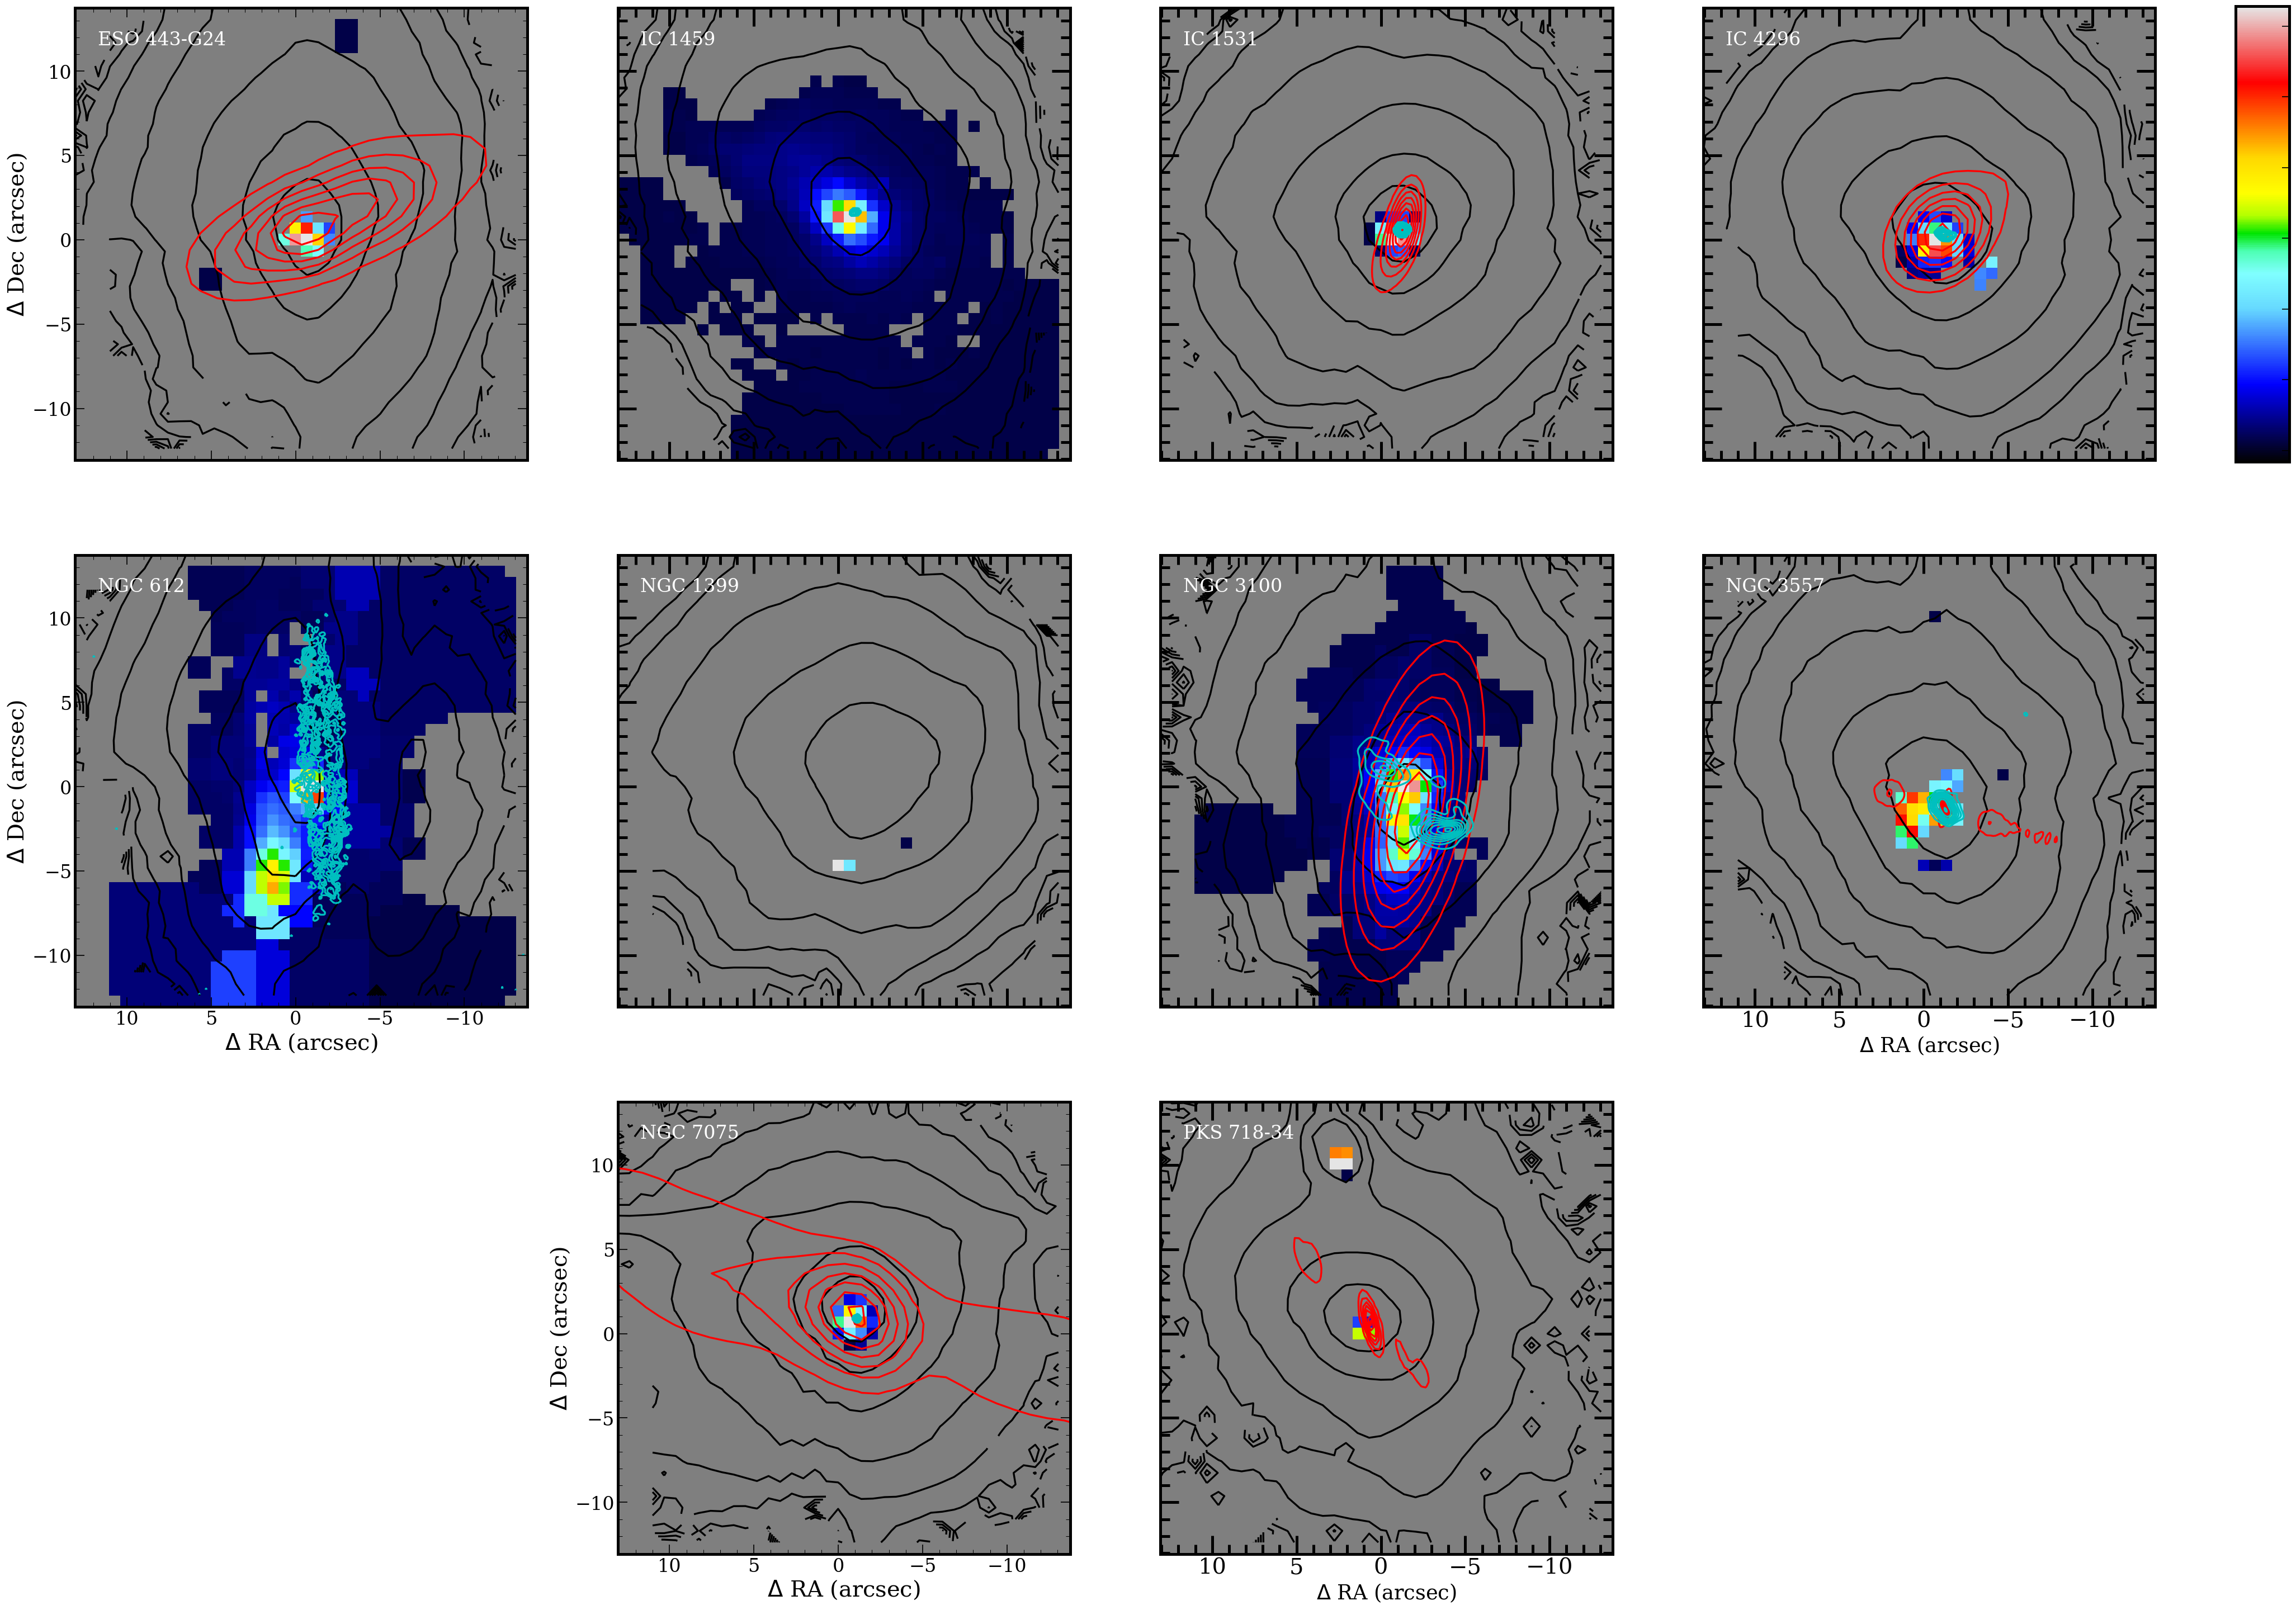
\includegraphics[width=\textwidth]{chapter5/vimos/Hb.png}
			\caption[VIMOS \bracket{\ion{O}{iii}} maps]{VIMOS [\ion{O}{iii}]$\lambda\lambda$4957,5007 maps. Total flux contours (isophotes) are shown in black, \ce{^{12}CO(2-1)} contours from ALMA in white, and radio continuum contours from VLA in green. The radio band shown depends on the spatial resolution and extent of the datasets available, selected to best match our IFS data.\label{fig:VIMOS_OIII}} 
			
		% \end{figure}
		% \begin{figure}
		% 	\centering
			\vspace{\floatsep}
			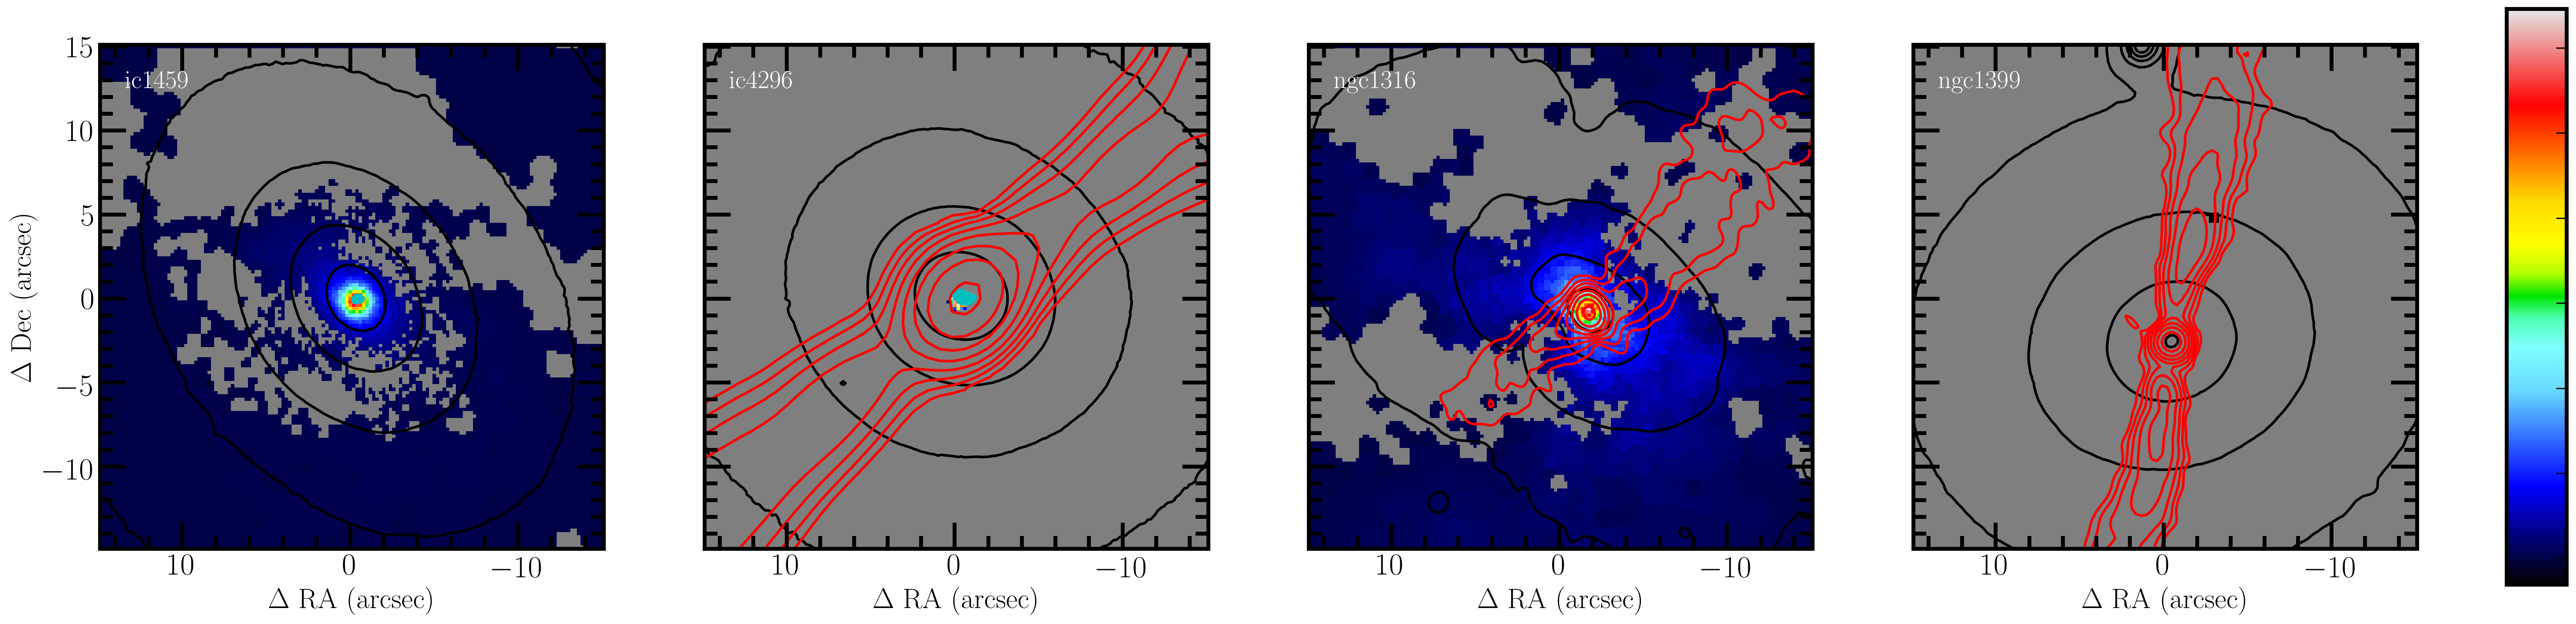
\includegraphics[width=\textwidth]{chapter5/muse/Hb.png}
			\caption[MUSE \bracket{\ion{O}{iii}} maps]{As in Fig.\ \ref{fig:VIMOS_OIII} but for MUSE [\ion{O}{iii}]$\lambda\lambda$4957,5007 maps.\label{fig:MUSE_OIII}} 
			
		\end{figure}

\begin{table}[t]
	\centering
\begin{threeparttable}
	\caption{Gas masses of the Southern Sample galaxies.}
	\label{tab:gasMass}
	% \begin{tabular*}{\textwidth}{@{\extracolsep{\fill}}l r r r l}
	\begin{tabular}{l c c c c}
		\hline
		\hline
		Galaxy & \multicolumn{2}{c}{\ion{H}{ii} Mass} & Balmer & LINER/ \\
		& VIMOS\tnote{a} & MUSE & Decrement & Seyfert \\
		& ($\log\mathrm{M_\odot}$) & ($\log\mathrm{M_\odot}$) & \\
		\hline
		ESO 443-G024 & $5.06 \pm 0.08$ 	& --  		& -- & LINER \\
		IC 1459 	& $5.21 \pm 0.07$	& $5.50 \pm 0.14$ & $4.53 \pm 2.64$ & LINER-AGN\\
		IC 1531 	& $5.09 \pm 0.11$	& -- 		& -- & Seyfert 2\\
		IC 4296		& $5.43 \pm 0.18$	& \tnote{b} & LINER-AGN \\
		NGC 612 	& $6.00 \pm 0.05$ 	& -- 		& -- & LINER-AGN \\
		NGC 1316 	& -- 				& \tnote{b} & LINER-AGN \\
		NGC 1399 	& $< 5.9$\tnote{c}	& $4.54 \pm 0.22$ & $>0.2$\tnote{c} & LINER \\
		NGC 3100 	& $5.26 \pm 0.06$	& -- 		& -- & LINER-AGN \\
		NGC 3557 	& $4.61 \pm 0.11$ 	& -- 		& -- & LINER \\
		NGC 7075 	& $4.68 \pm 0.08$	& -- 		& -- & LINER \\
		PKS 718-34  & $< 6.4$\tnote{c} & -- & -- & Passive \\
		\hline
		\hline
	\end{tabular}
	\begin{tablenotes}
	\footnotesize
	\note Col.\,1: Galaxy. Col.\,2: \ion{H}{ii} mass derived from the H$\beta$ line in the VIMOS data, assuming a Balmer decrement of 2.85. Col.\,3: \ion{H}{ii} mass derived from the H$\alpha$ line in the MUSE data. Col.\,4: Balmer decrement measured from the MUSE data. Col.\,5: Main source of ionizing radiation (see Section \ref{sec:Diagnostics} for a description of the different classes). -- means we have no data.
	\item [a] The VIMOS flux calibration and thus the derived gas masses are only approximate (see Section \ref{subsec:VIMOSreduction} for more detail on the flux calibration).
	\item [b] Both H$\alpha$ and H$\beta$ are not detected with A/N $>2.5$, so no information can be gained.
	\item [c] H$\beta$ is not detected with A/N $> 2.5$, so the fit is unreliable. Instead the limits for a 2.5 A/N detection are shown.
	\end{tablenotes}
\end{threeparttable}
\end{table}

		As can be seen from Fig.\,\ref{fig:VIMOS_OIII}, both NGC 612 and NGC 3100 have significant off-centre clouds of ionized gas. The latter is spatial coincident with both the radio jet and the gap in the CO ring (this is discussed further in Section \ref{subsec:BPT}), while former seems to have no link with either the radio jet (a massive jet extending $\sim 200$\,kpc to the east and west of the galaxy centre) or the CO. 

		It was considered that a similar analysis to that of Sections \ref{subsubsec:RobustKin} and \ref{subsubsec:RobustAbs} to compare the radial profiles for the [\ion{O}{iii}] and H$\beta$ fluxes might have been some use to test the robustness of the reduction of the VIMOS datacubes, however given that the final VIMOS flux calibration was done using the MUSE datacubes a comparison is somewhat nonsensical. The H$\alpha$ (MUSE) and H$\beta$ (VIMOS) radial profiles are shown later in Figs.\,\ref{fig:Ha_profile_MUSE} and \ref{fig:Hb_profile_VIMOS} and all show a profile which is proportional $r^2$.


		% \subsubsection{Robustness of Emission Line Results}
		% 	\label{subsubsec:RobustEmi}

		% 	Here as in Sections \ref{subsubsec:RobustKin} and \ref{subsubsec:RobustAbs} we examine the robustness of the results by comparing the values of parameters derived by the VIMOS and MUSE datasets. Figures \ref{fig:compare_ic1459} and \ref{fig:compare_ic4296} show the fluxes measured from the best-fitting emission lines for [\ion{O}{iii}] and H$\beta$ from each dataset is consistent with each other. While this test is a little redundant, given that the VIMOS fluxes are calibrated using the MUSE fluxes, it is still important to show that in the case of IC 1459, which has significant extended ionized gas, the radial profile has a consistent shape between the two instruments.

		% 	\begin{figure}
		% 		\centering
		% 		\includegraphics[width=.9\textwidth]{chapter5/compare_ic1459.png}
		% 		\caption[Comparison between emission line radial profiles from VIMOS and MUSE datacubes for IC 1459]{A comparison of the emission lines for VIMOS (red) and MUSE (blue) datasets for IC 1459.}
		% 		\label{fig:compare_ic1459}
		% 	\end{figure}

		% 	\begin{figure}
		% 		\centering
		% 		\includegraphics[width=.9\textwidth]{chapter5/compare_ic4296.png}
		% 		\caption[Comparison between emission line radial profiles from VIMOS and MUSE datacubes for IC 4296]{A comparison of the emission lines for VIMOS (red) and MUSE (blue) datasets for IC 4296.}
		% 		\label{fig:compare_ic4296}
		% 	\end{figure}



	\subsection{Gas Masses}
		\label{subsec:GasMass}

		Total ionized gas masses are derived using the prescription of \citet{Sarzi2005}. This is a very rough calculation and the values should not be used for quantitative applications. The approach follows \citet{Kim1989}, whereby
		\begin{equation}
			\left(\frac{M_\text{\ion{H}{ii}}}{M_\odot}\right) = 280 \left(\frac{D}{10\, \mathrm{Mpc}}\right)^2 \left(\frac{F(\mathrm{H\alpha})}{10^{-14} \, \mathrm{erg \, s^{-1} \, cm^{-2}}}\right) \left(\frac{10^3 \, \mathrm{cm^{-3}}}{n_\mathrm{e}}\right) \, ,
		\end{equation}
		where $M_\text{\ion{H}{ii}}$ is the total mass of \ion{H}{ii} in the galaxy, $D$ is the galaxy distance, and $F(\mathrm{H\alpha})$ is the H$\alpha$ flux measured from the spectrum created by summing spatially all spaxels within an aperture of $\frac{R_\mathrm{e}}{2}$ (chosen to exclude noisy outer regions of the observations, but still include the bulk of the gas in systems with significant spatially-extended gas). This method assumes an electron density $n_\mathrm{e} = 100 \, \mathrm{cm^{-3}}$, a temperature of $10^4$ K and case-B recombination (photons above 13.6\,eV are reabsorbed by the gas, photoionizing a nearby neutral Hydrogen atom, thus not affecting the overall ionization state; e.g.\ \citealt[p.\,74]{Osterbrock1974}). For VIMOS data we use the Balmer decrement such that $\amthrm{H}\alpha = 2.86 \mathrm{H}\beta$ (the Balmer decrement is discussed further in Section \ref{subsec:Ndec}). Like \citet{Sarzi2005}, we only claim a detection if the amplitude-to-noise ratio (A/N) is $>4$ for [\ion{O}{iii}] and $>2.5$ for H$\beta$ or H$\alpha$ lines for VIMOS and MUSE data, respectively. When these conditions are not met, upper limits are calculated using the 2.5 A/N level, assuming the gas has the same velocity dispersion as the stellar component.

		Our calculated gas masses are given Table \ref{tab:gasMass} and are at the upper limit of, and possibly exceed, the typical masses observed in ETGs. Given that our sample contains particularly massive galaxies, high ionized gas masses are not unexpected, however.

\section{Ionized Gas Kinematics}
	\label{sec:GasKin}
	In Figs.\,\ref{fig:VIMOS_Gaskine} and \ref{fig:MUSE_Gaskine}, we show maps of the mean velocity and velocity dispersion of the ionized gas for the 4 galaxies with extended emission lines, IC 1459, NGC 612, NGC 1316 and NGC 3100. Due to that fact that, unlike stars, gas is dissipational, it is to be expected that given sufficient time, the ISM will always settle into a disc. These maps show that the warm component of the ISM of the Southern sample galaxies varies from largely settled discs in IC 1459 and NGC 612 to more disordered kinematics of NGC 3100 and a possible inflow in NGC 1316.

	\begin{figure}
		\centering
		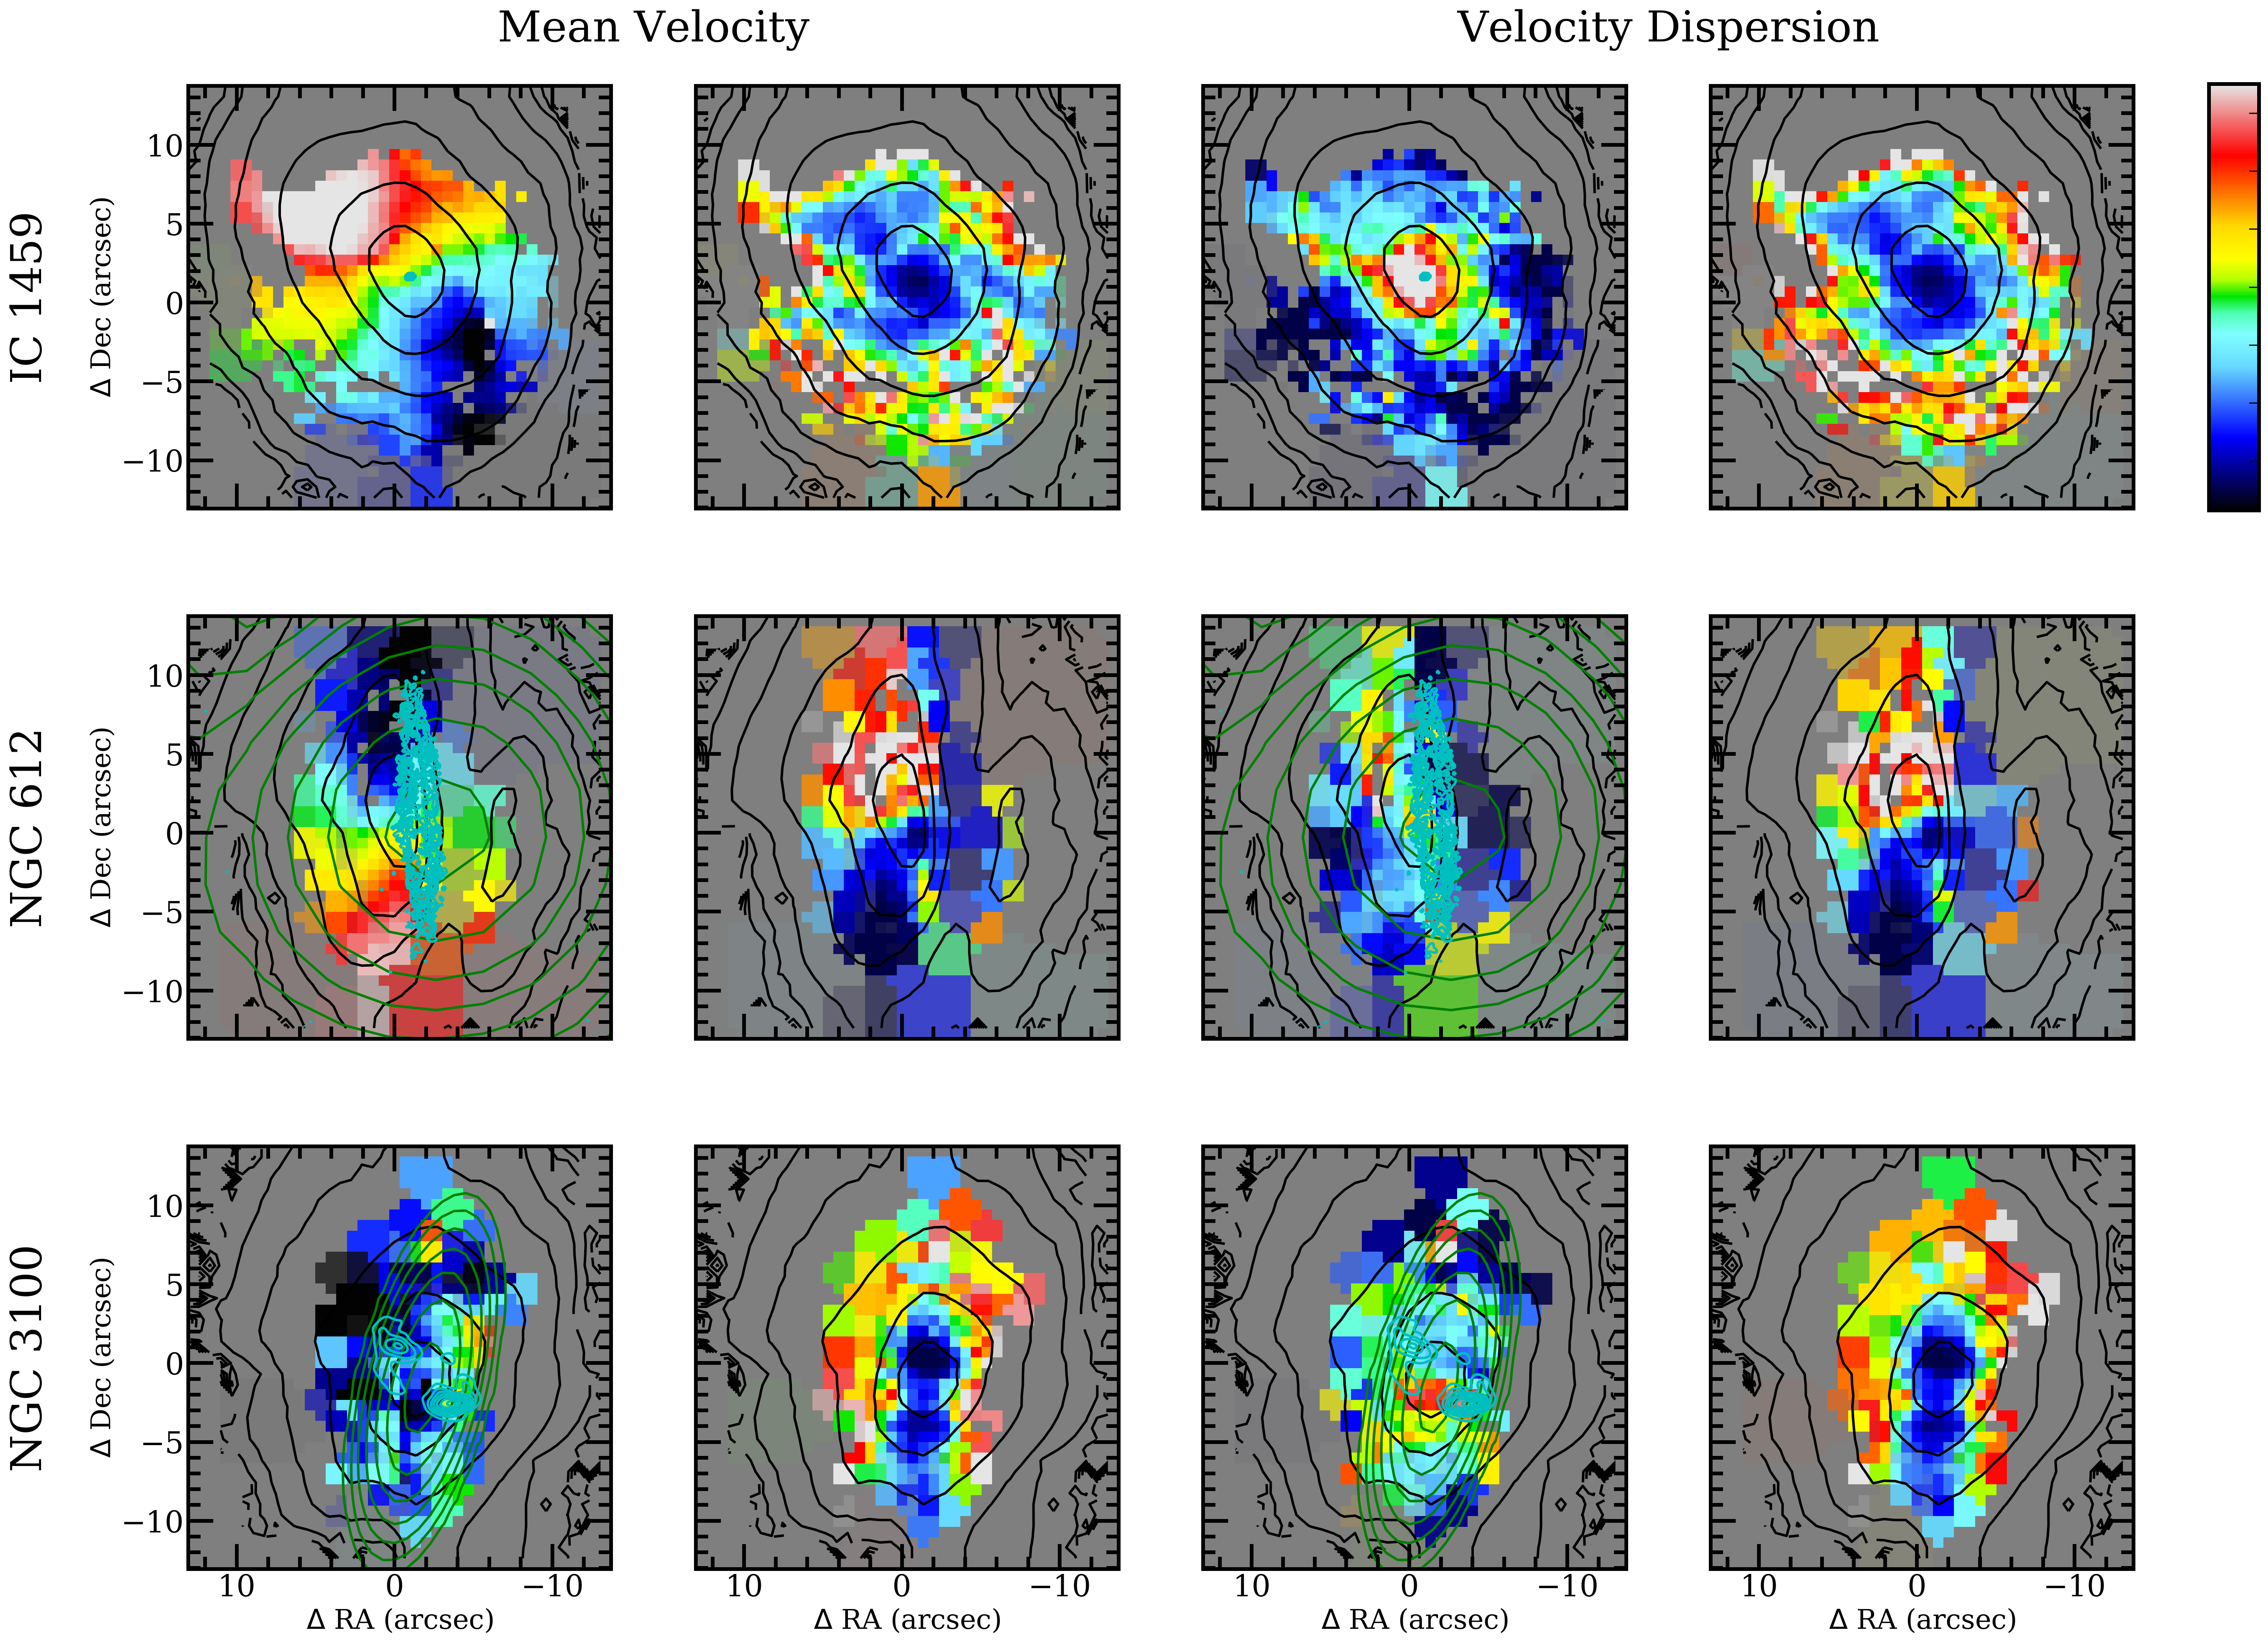
\includegraphics[height=0.47\textheight]{chapter5/vimos/kin.png}
		\caption[VIMOS ISM kinematic maps]{VIMOS ISM kinematic maps. Left to right: mean velocity and velocity dispersion maps. Alternate columns show a given parameter and its associated uncertainty. Top to bottom: IC 1459, NGC 612 and NGC 3100. Contours are as in Fig.\ \ref{fig:VIMOS_OIII}. Colour scale ranges are: mean velocity maps -360 to 360\,$\mathrm{km \, s^{-1}}$ (except for NGC 3100 which has a range of -100 to 100\,$\mathrm{km \, s^{-1}}$), mean velocity uncertainty 1 to 15\,$\mathrm{km \, s^{-1}}$, velocity dispersion 35 to 200\,$\mathrm{km \, s^{-1}}$, and velocity dispersion uncertainty 1 to 20\,$\mathrm{km \, s^{-1}}$.} 
		\label{fig:VIMOS_Gaskine}
	\end{figure}

	\begin{figure}
		\centering
		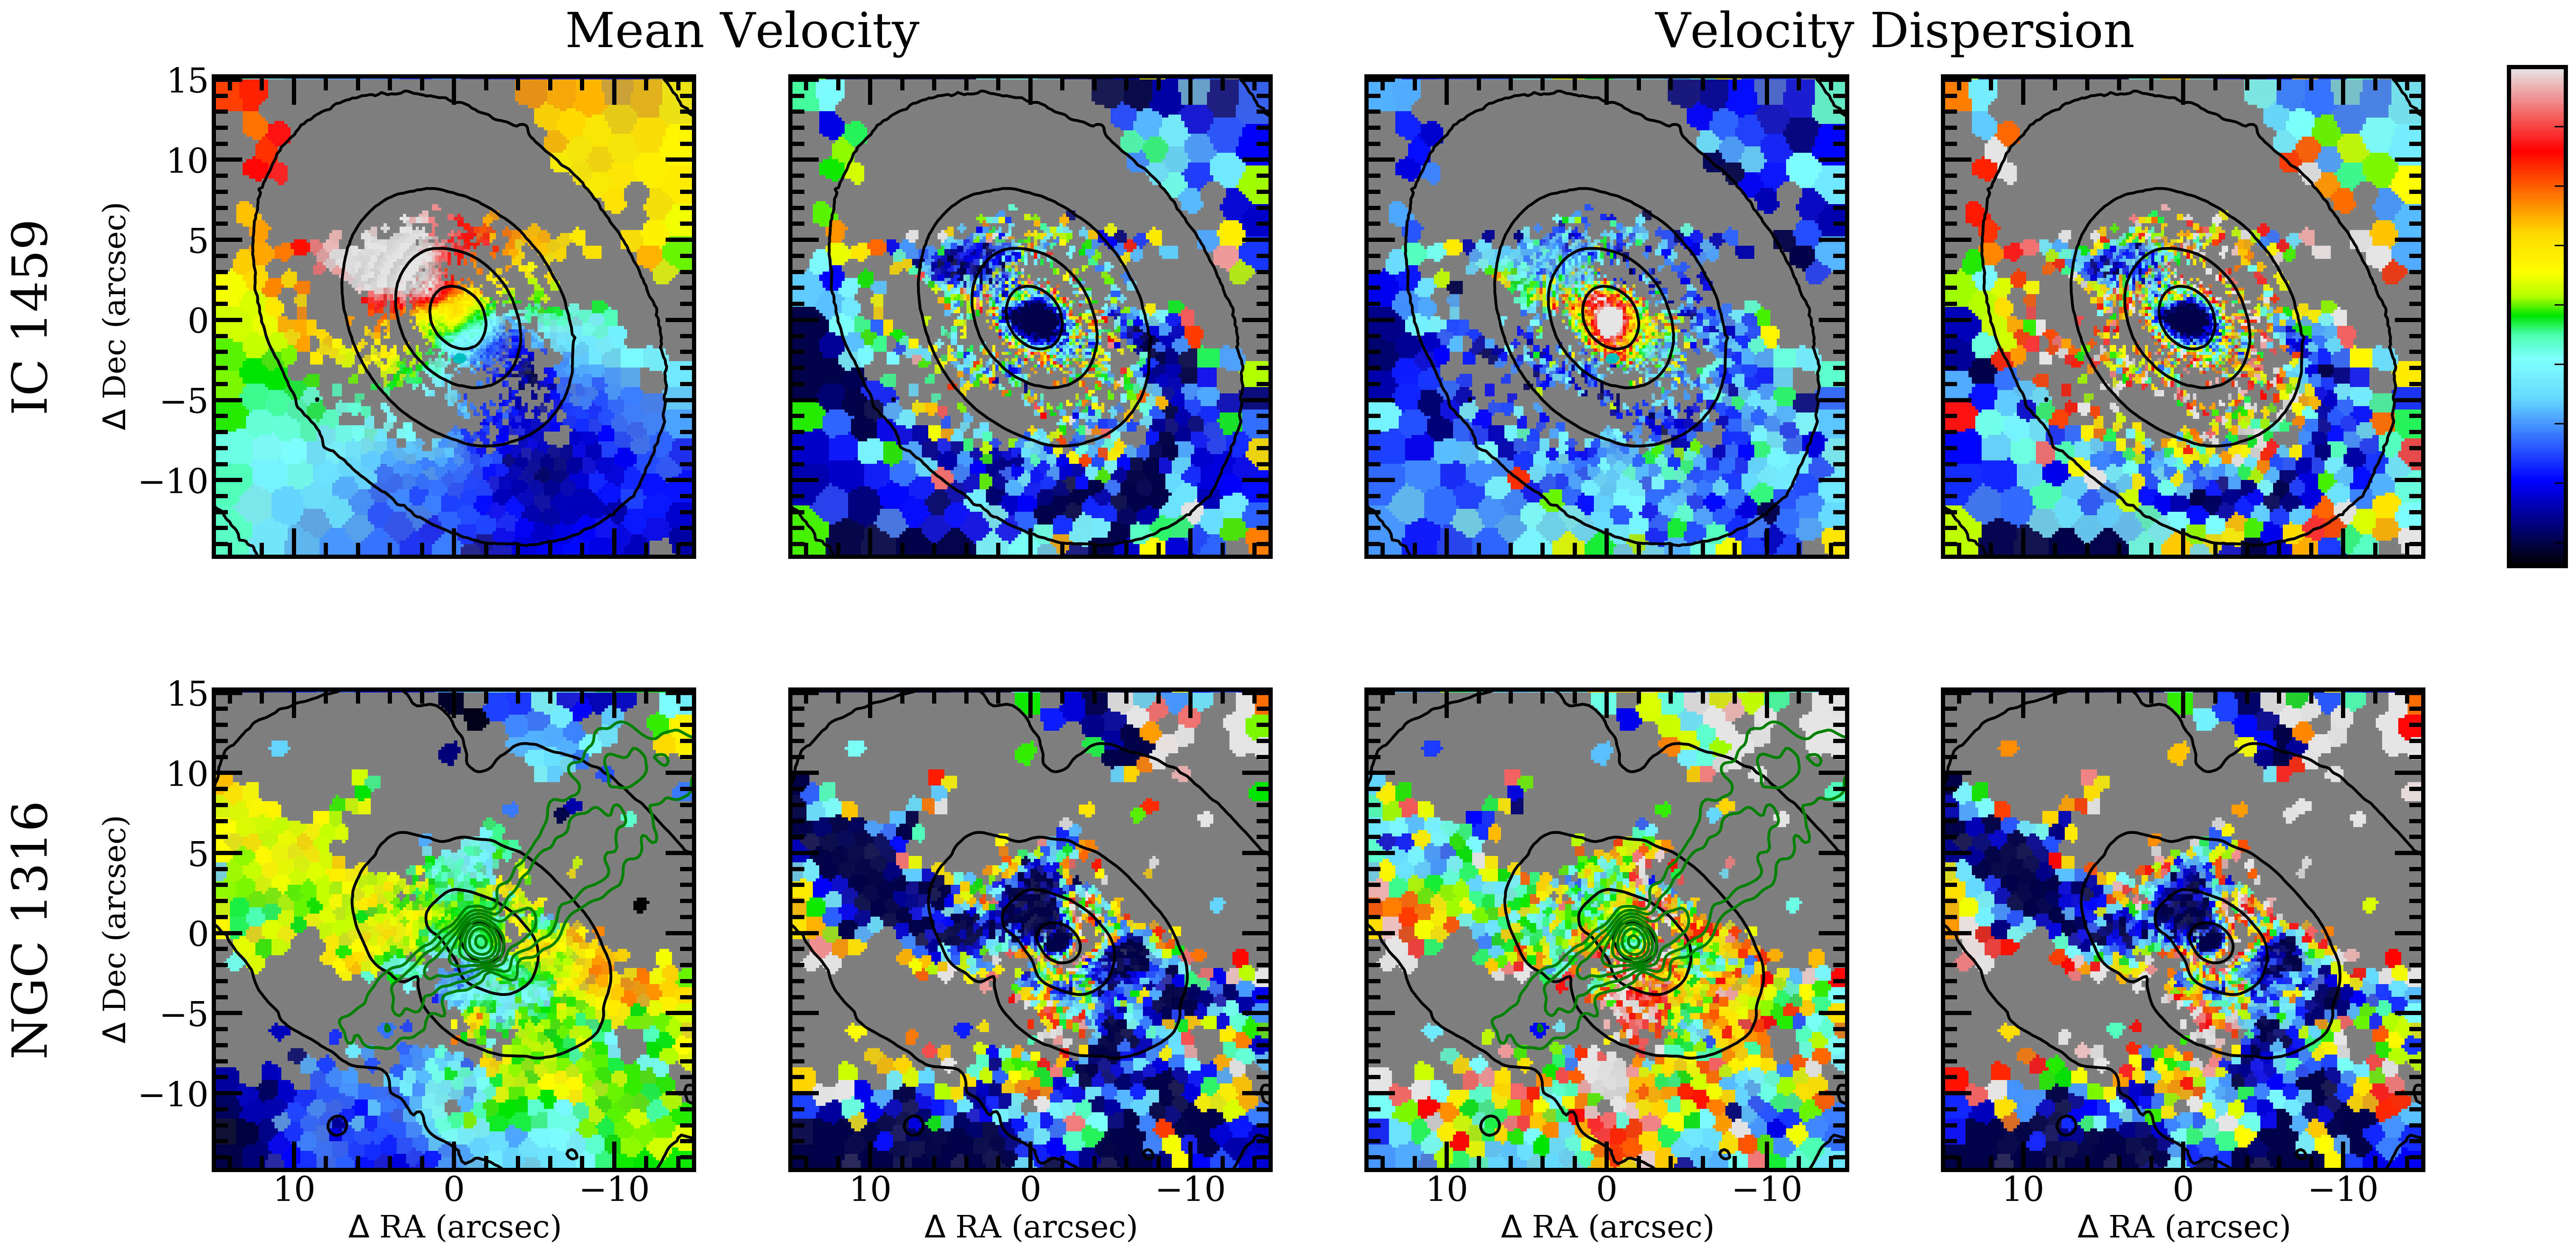
\includegraphics[height=0.31\textheight]{chapter5/muse/kin.png}
		\caption[MUSE ISM kinematic maps]{As Fig.\ \ref{fig:VIMOS_Gaskine} but for the MUSE ISM kinematics.}
		\label{fig:MUSE_Gaskine}
	\end{figure}


% Separate section?
	% \subsection{Misalignment of Gas}
	% 	\label{subsec:Gasmisaligment}
	It is immediately clear when comparing the stellar mean velocity maps (Figs.\,\ref{fig:VIMOS_stellar} and \ref{fig:MUSE_stellar}) to the ionized gas mean velocity maps (Figs.\,\ref{fig:VIMOS_Gaskine} and \ref{fig:MUSE_Gaskine}) that where gas is detected, its angular momentum is not often aligned with that of the stars. A misalignment between the kinematics of the stars and gas suggests an external origin for the gas (e.g.\ accretion or wet merger). However it should be noted that the converse is not necessarily true: aligned kinematics is consistent with an internal origin (e.g.\ stellar-mass loss), but it does \emph{not} require it \citep[e.g.][]{Davis2011a}. 

	We now comment on each galaxy in turn.

	\paragraph{IC 1459} has ionized gas counter-rotating with respect to the stellar kinematically-decoupled core, and also rotating independently from the rest of the galaxy. \citet{Franx1988} claim that the rotation of the gas is aligned with that of the stars outside of the KDC, however we observe outer stellar kinematics to be non-rotating. As the stellar disc did not survive the merger even that created the KDC, it is unlikely that the gas in IC 1459 progenitor galaxy survived. The lost gas may, however, have been re-accreted. Alternatively, the ISM may have yet another external origin. 

	\paragraph{NGC 612} has well aligned stellar and gaseous kinematics. The misalignment between the position angle of the stellar and gas kinematics (using the method described in Section \ref{subsec:Misalignment}) is just $1\fdg0\pm0\fdg7$, consistent with an internal origin for the gas. This adds to the evidence (see Appendix \ref{cha:Description}) that NGC 612 has not undergone a recent major merger (major mergers exhaust galaxies of their gas and destroy a stellar disc; see Section \ref{sec:stellarDiscussion}) and suggests that, the fuelling and powering of the radio jet could be a purely secular process. 


	\paragraph{NGC 1316} is a complex object. Since there are redshifted emission lines with respect to the rest frame of the galaxy on both sides of the galaxy, the gas is not in a settled disc and that there must be some inflow/outflows. From visual inspection of the velocity field for the gas (Fig.\,\ref{fig:MUSE_Gaskine}) it is clear that a simple exponential disc model will not be well fitted to the data. We suggest that that the large velocity peak on the southwest side of the galaxy could be an inflow towards the nucleus, almost perpendicular to the radio jet, however we acknowledge that other interpretations are possible. Better quality data (longer exposure times) and more sophisticated models are required to add certainty to this interpretation. Nevertheless, it is clear that the gas in not in a settled disc. 


	\paragraph{NGC 3100} has an interesting ISM morphology. The \ce{^{12}CO(2-1)} contours (shown in white in all figures) show a broken ring with the radio jet passing through the gaps in the ring (Ruffa et\,al., in prep.). We observe the ionized gas to be brightest in the gaps of this ring which we interpret as additional excitation of the gas due to shocks from the impact of the jet (discussed in more detail in Section \ref{subsec:BPT}). The simplest comment that we can make of the ionized gas kinematics is that it is completely different than that of the stars. Secondly, that the centre of rotation of the gas appears to be offset from the centre of the galaxy (as defined by the stellar surface brightness) by several arcseconds to the west. 

	\subsection{Kinematic mis-alignments}
		\citet{Davis2011a} showed that $36\pm5$\% of fast rotators have ionized gas kinematics misaligned with respect to the stellar kinematics, while slow rotators have a flat distribution with respect to their misalignment angles \citep[see fig.\ 4]{Davis2011a}. This indicates that slow rotators are dominated by external sources of gas, while fast rotators can have either internal or external sources. This is consistent with our observations of the Southern Sample: the only slow rotator with detected ionized gas is IC 1459, which has significantly kinematically-misaligned gas; while of the 3 fast rotators, only 1 (NGC 3100) is definitely misaligned, while NGC 612 is consistent with an internal gas origin and NGC 1316 is unclear.

\section{Ionization Sources}
	\label{sec:Diagnostics}
	Determining the sources of ionizing radiation in galaxies using emission line ratios, such as Baldwin\,--\,Phillips\,--\,Terlevich (BPT) plots (\citealt{Baldwin1981}; revised by \citealt{Kewley2001, Kewley2006} and \citealt{Kauffmann2003a}), has become an increasingly widespread exercise. That said, there are several important caveats. Firstly, great care must be taken when applying each diagnostic; much of the literature misinterprets the resulting classifications. Secondly, in the absence of spatially-resolved spectra, low-ionization nuclear emission-line region (LINER) classifications have often been taken as a marker for jet-mode active galactic nuclei (AGN). As discussed in Section \ref{subsubsec:JetFeedback} however, several recent surveys have shown that many of these may not be bona-fide AGN \citep[e.g.][]{Sarzi2005, Sarzi2010, Singh2013, Belfiore2016a}. In these cases, the emission may not even originate exclusively from the centres of the galaxies, the location of the putative AGN. This led to the creation of the low-ionization emission-line region (LIER) classification, with the same criteria as LINERs, but not necessarily restricted to the nuclear regions.

	The problem with classifying ETGs by their emission lines is that they often have very little ionized gas and weak ionizing radiation fields, so that it is often difficult to detect emission lines from their ISM. Furthermore, the BPT plots require a larger spectral range than many integral-field spectrographs (IFS) deliver. This has given rise to a number of other, analogous, classifying plots, that we take advantage of here. A description of our ionization source classifying process follows below. 

	Firstly, we preferentially use the BPT plots for the galaxies observed with MUSE (MUSE has the required spectral range; see Section \ref{subsec:BPT}). This allows us to classify galaxies into star-forming, LINER/LIER or Seyfert 2 classes. For the emission-line fluxes derived from the VIMOS datacubes, we use the [\ion{N}{i}]/H$\beta$ versus [\ion{O}{iii}]/H$\beta$ plot of \citet[hereafter the SAURON plot]{Sarzi2010}. Unlike the BPT plots, \citet{Sarzi2010} do not define classification boundaries. In Section \ref{subsec:Ndec} we find a linear relationship between [\ion{N}{ii}]/H$\alpha$ and [\ion{N}{i}]/H$\beta$ using our archival MUSE observations. We exploit this to transform the classification boundaries of the classic BPT [\ion{N}{ii}]/H$\alpha$ versus [\ion{O}{iii}]/H$\beta$ to the SAURON diagnostic plot. %We use the Balmer decrement (see Section \ref{subsec:Ndec}) and the [\ion{N}{i}] flux versus [\ion{N}{ii}] flux relation (Section \ref{subsec:Ndec}) to convert the [\ion{N}{ii}]/H$\alpha$ BPT plot classification boundaries of \citet{Kewley2001} and \citet{Kauffmann2003a} to the [\ion{N}{i}]/H$\beta$ SAURON plot (as described in more detail in Section \ref{subsec:Ndec}). 
	This allows us to classify galaxies into star-forming or LINER/Seyfert 2 classes. We also use the so-called WHaN2 plot (H$\alpha$ equivalent width versus [\ion{N}{ii}]/H$\alpha$; see Section \ref{subsec:WHaN2}) from \citet{CidFernandes2011}. Using a similar method as above, we transform this plot into a H$\beta$ equivalent width versus [\ion{N}{i}]/H$\beta$ (WHbN1) plot for the VIMOS data, by finding a linear relationship between the H$\alpha$ to the H$\beta$ equivalent widths using our archival MUSE observation (again described in more detail in Section \ref{subsec:Ndec}). %To transform the equivalent widths of H$\alpha$ to H$\beta$, we find the continuum at H$\alpha$, $C_\text{6563\AA}$, and plot it against the continuum at H$\beta$, $C_\text{4861\AA}$ (again described in more detail in Section \ref{subsec:Ndec}). 
	This allows us to classify galaxies into star-forming, strong AGN (Seyfert 2), weak AGN (LINER) or retired classes. 

	To check if the LINER classifications are due to a central radiation source (such as an AGN) or extended sources (such as weak star formation or post-asymptotic giant branch stars; pAGB stars), we examine the H$\alpha$ and H$\beta$ flux radial profiles of our galaxies with extended detected ionized gas (Section \ref{subsec:Hb}). Finally, in Section \ref{subsec:MEx} we use the mass\,--\,excitation (MEx) plot of \cite{Nyland2016}, using parameters derived from the spatially-integrated spectra within an aperture of radius 3\arcsec, thus only probing the central region of the galaxies. This allows us to classify into star-forming, Seyfert 2, LINER, transition or passive classes, and subdivide LINER galaxies into those whose LINER characteristics are attributable to a central AGN (labelled LINER-AGN) and those whose LINER characteristics are not. 

	% \subsection{Using Emission Line Beyond the VIMOS Wavelength Range}
	\subsection{Extrapolating VIMOS Data}
		\label{subsec:Ndec}
		\begin{figure}
			\centering
			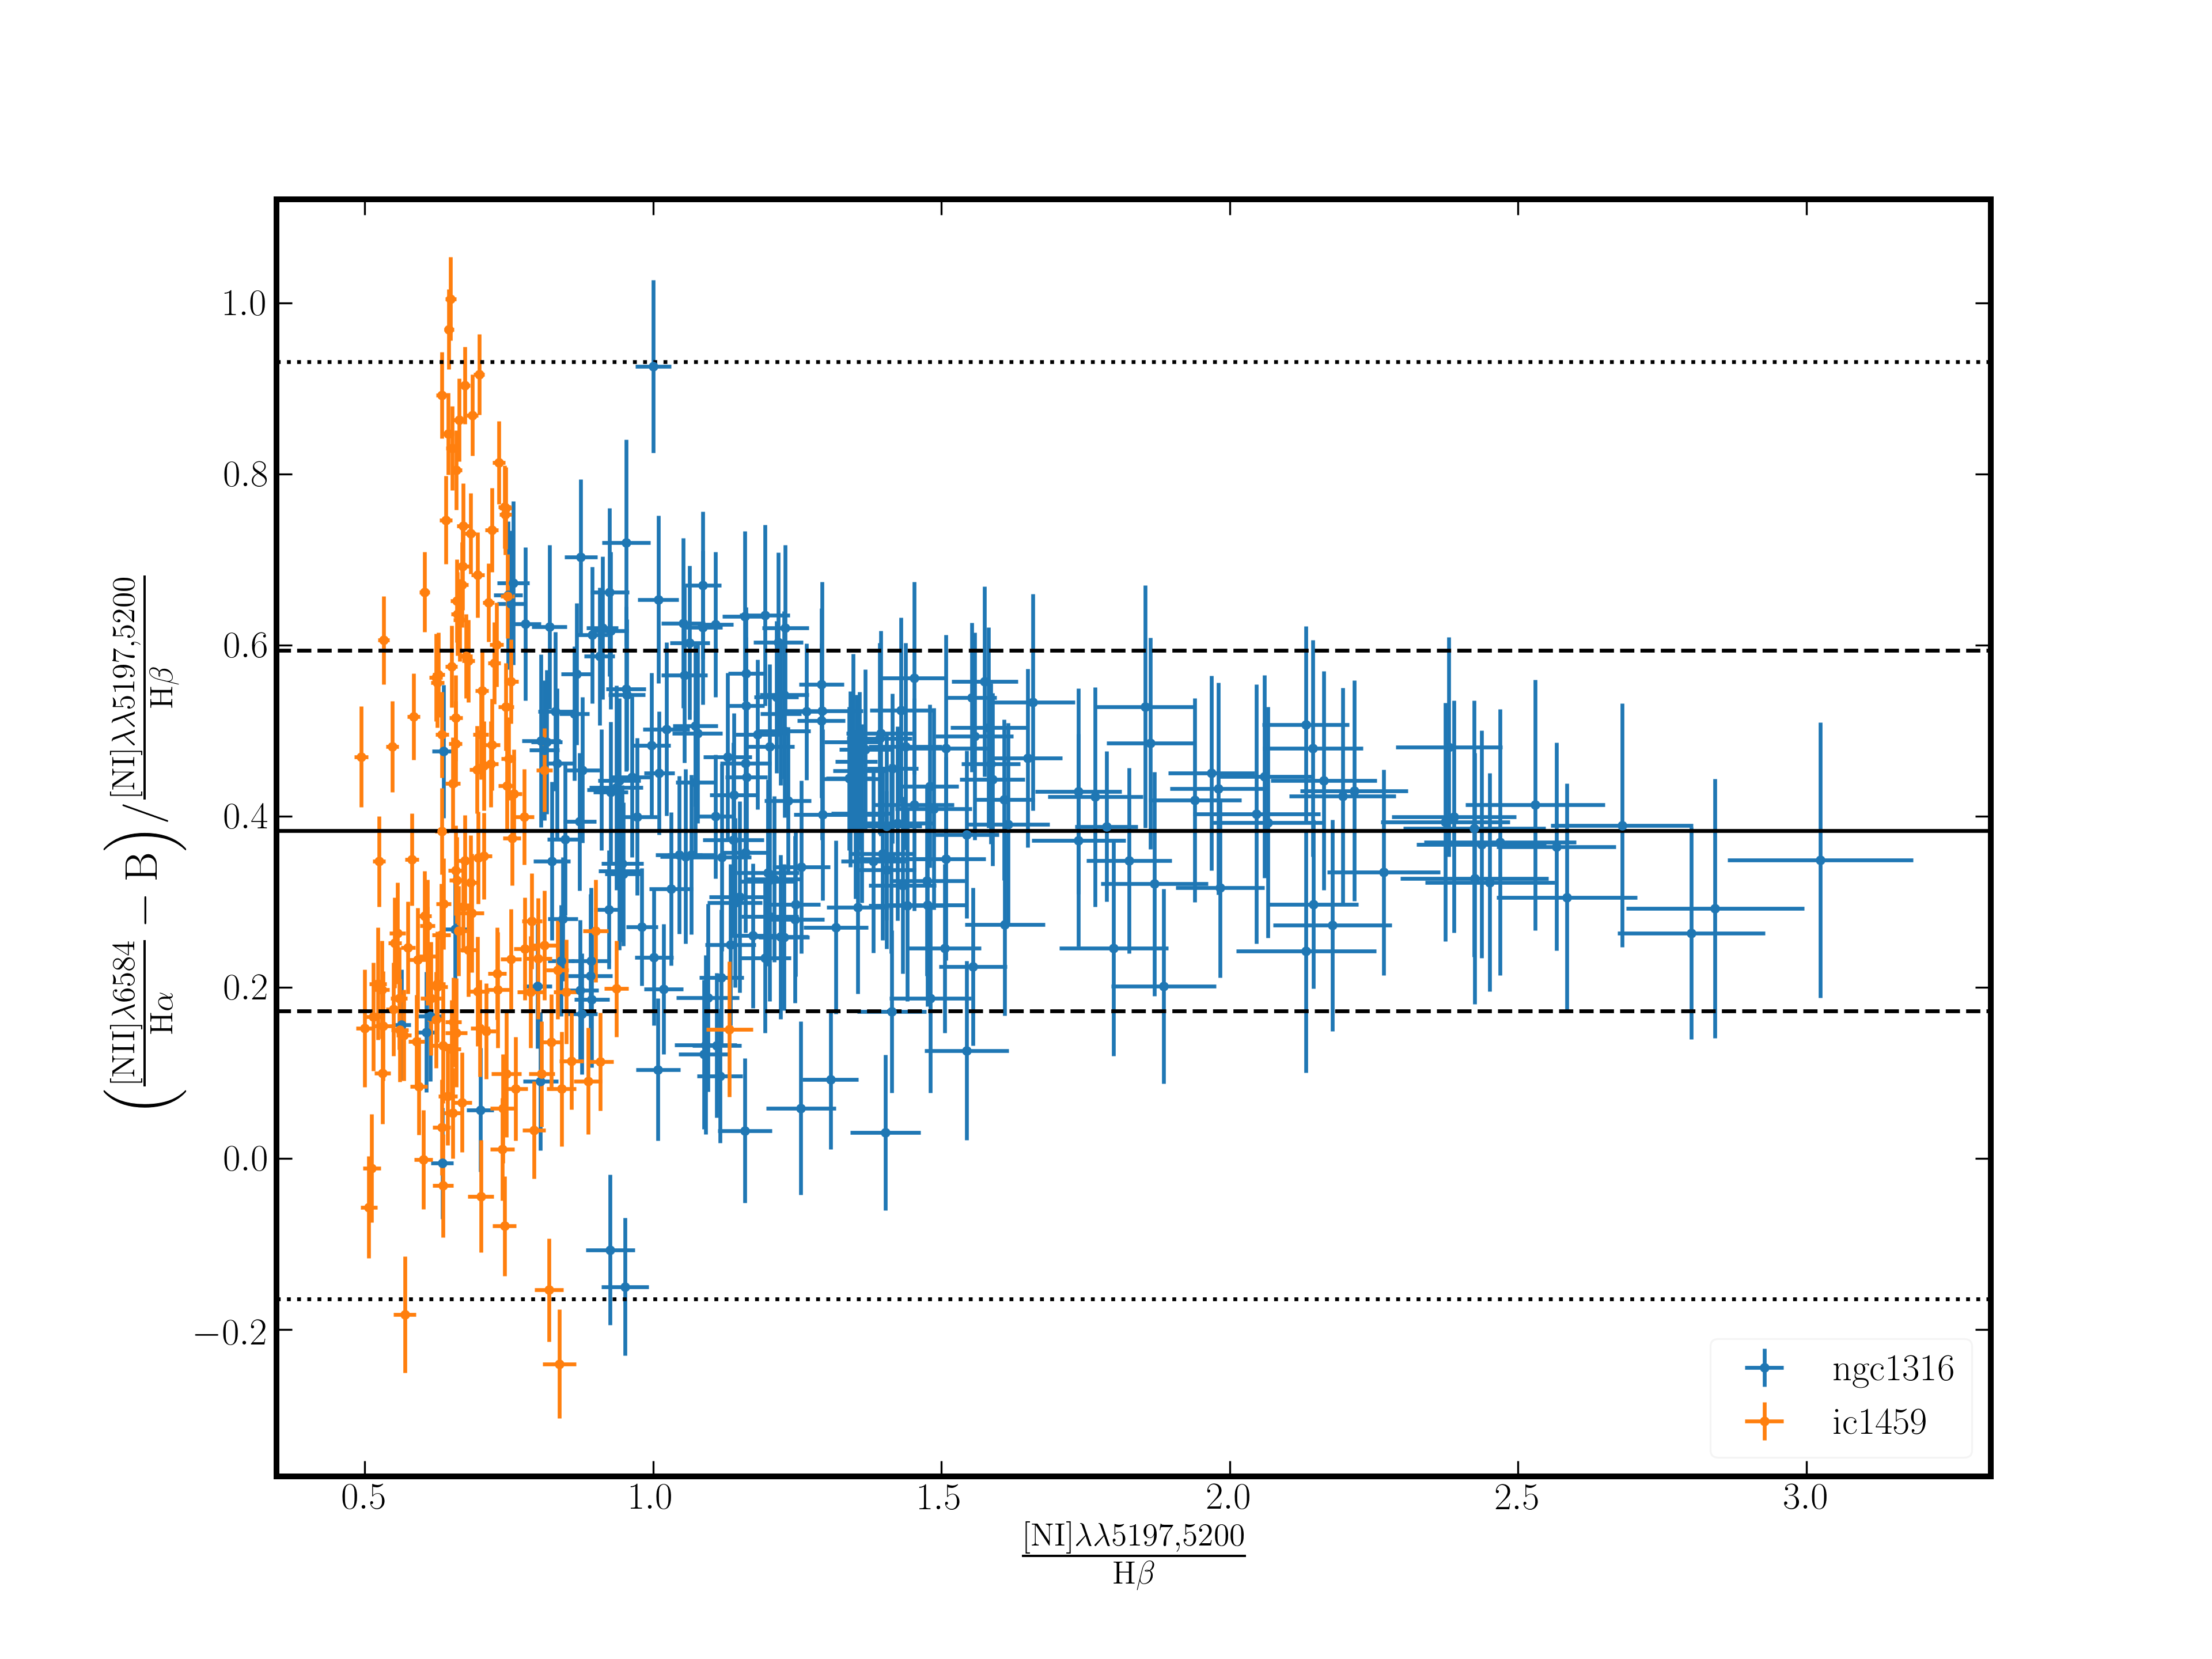
\includegraphics[width=0.55\textwidth]{chapter5/ratio_fit.png}
			\caption[\bracket{\ion{N}{ii}}/H$\alpha$ vs \bracket{\ion{N}{i}}/H$\beta$]{Upper panel: [\ion{N}{ii}]/H$\alpha$ vs [\ion{N}{i}]/H$\beta$ line ratios for the galaxies IC 1459 and NGC 1316, used to transform the classification boundaries e.g.\ the classic [\ion{N}{ii}] BPT plot to the SARUON diagnostic plot. Lower panel: Residuals = ([\ion{N}{ii}]/H$\alpha$ - best-fit)/[\ion{N}{i}]/H$\beta$. The solid line shows the best-fitting (Eq.\ \ref{eq:N_dec}) in both panels, while the dashed and dotted lines show the 68 and 99 percentiles, respectively.\label{fig:ratio_relation}}
		% \end{figure}

		% \begin{figure}
		% 	\centering
			\includegraphics[width=0.55\textwidth]{chapter5/EQw_fit.png}
			\caption[Comparing H$\alpha$ and H$\beta$ equivalent widths]{Upper panel: H$\alpha$ vs H$\beta$ equivalent widths for the galaxies IC 1459 and NGC 1316 used to transform the classification boundaries of diagnostics involving the H$\alpha$ equivalent width to those involving H$\beta$. Lower panel: Residuals = (EW(H$\alpha$) - best-fit)/EW(H$\beta$). The solid line shows the best-fitting (Eq.\ \ref{eq:EqW_dec}) in both panels, while the dashed and dotted lines show the 68 and 99 percentiles, respectively.\label{fig:EqW_relation}}
		\end{figure}

		The Balmer decrement, $d_\mathrm{H}$, is the ratio of the H$\alpha$ to H$\beta$ fluxes. There are good theoretical motivations for this ratio to be near constant at $d_\mathrm{H} = 2.86$, under a wide variety of conditions. In reality, however, higher values are routinely observed. These can be explained as due to either the presence of dust causing extinction (whereby emission lines at shorter wavelengths appear dimmer than expected from their redder counterparts due to dust preferentially scattering and absorbing bluer light) or some mechanism that populates hydrogen levels from the ground up. Such mechanisms may be important in high-density environments, such as within powerful (type 1) AGN \citep[e.g.][]{Shields1974, Netzer1975}. 
		%
		% The majority ($\approx 60$\%) of ETGs and all LINER and Seyfert galaxies are dusty \citep[e.g.][]{Martini2013}. 
		% Such galaxies reveal clear dust lanes in \textit{Hubble Space Telescope (HST)} observations \citep[e.g.][]{Martini2013}, are bright in the infrared (where the thermal emission from dust is seen as a dust ``bump''; e.g.\ \citealt{Jura1987, Knapp1992}), and possess other emission lines \citep[e.g.\ \bracket{\ion{S}{ii}};][]{Wampler1968} showing similar reddening. Thus, assuming the observed steepening of the Balmer decrement is entirely due to dust, the ratio of the observed decrement to the theoretical value of 2.86 is a good estimate of the dust reddening.

		If we assume that different ionization states of a given atomic species occur in the same spatial location, then shielding is not important or at least is not non-linear in its effect on the emission-line ratios. Given that the different states are then produced under the same conditions, it is natural to expect a simple relationship between their emission line fluxes, similar to the Balmer decrement. We exploit such relationships to transform classification boundaries from diagnostic plots which use emission lines outside of the spectral range of VIMOS to diagnostics which can be measured with our VIMOS data e.g.\ transform from the classic BPT [\ion{N}{ii}]/H$\alpha$ versus [\ion{O}{iii}]/H$\beta$ to [\ion{N}{i}]/H$\beta$ versus [\ion{O}{iii}]/H$\beta$ diagnostic plot (hereafter the SAURON diagnostic plot) of \citet{Sarzi2010}. We achieve this by finding a best-fitting relationship between the relevant measurements taken in each bin of the galaxies for which we have the relevant detections in our MUSE data (due to the lack of detectable emission line in the observations of IC 4296 and NGC 1399, we therefore use the observations of IC 1459 and NGC 1316). This relationship is then applied to the diagnostic boundary lines in the relevant plots below. We emphasize that these are purely empirical relationships and thus differ substantially from the Balmer decrement with its strong theoretical basis (although these relationships include the effect of the Balmer decrement). 

		The two transformations that we use are from [\ion{N}{ii}]/H$\alpha$ to [\ion{N}{i}]/H$\beta$ line ratios and from the H$\alpha$ to the H$\beta$ equivalent widths. In both cases we fit a linear relationship $y = Ax + B$ using the least-trimmed squares routine, \textsc{lts\_linefit}\footnote{http://www-astro.physics.ox.ac.uk/\~mxc/software/\#lts} of \citet{Cappellari2013} due to its robust handling of the uncertainties along both axes. These are shown in Figs.\ \ref{fig:ratio_relation} and \ref{fig:EqW_relation}, where we find
		\begin{align}
			\frac{[\text{\ion{N}{ii}}]}{H\alpha} & = \, (0.38 \pm 0.02) \frac{[\text{\ion{N}{i}}]}{H\beta} + (1.80 \pm 0.02)
			\intertext{and}
			\mathrm{EW}(H\alpha) & = \, (2.92 \pm 0.03) \mathrm{EW}(H\beta) - (0.16 \pm 0.02) \, ,
				\label{eq:EqW_dec}
			\intertext{respectively. Since it is sometimes observed that [\ion{N}{ii}]/H$\alpha < 1.80$, which if blindly applying the relationship found above, results in an unphysical [\ion{N}{i}]/H$\beta < 0$ (i.e.\ negative flux), we instead rearrange and use}
			\frac{[\text{\ion{N}{i}}]}{H\beta} & = \, 
			\begin{cases}
				(0.38 \pm 0.02) \frac{[\text{\ion{N}{iI}}]}{H\alpha} + (1.80 \pm 0.02), & \text{if}\ \frac{[\text{\ion{N}{ii}}]}{H\alpha} < 2 \\
				(0.38 \pm 0.02) \frac{[\text{\ion{N}{ii}}]}{H\alpha}, & \text{otherwise.}
			\end{cases}
			\label{eq:N_dec}
	\end{align}


	\subsection{BPT Diagnostics}
		\label{subsec:BPT}
		Firstly, in Fig.\,\ref{fig:BPT}, we examine our galaxies using the classic BPT diagnostic plots. For the plots using [\ion{N}{ii}]/H$\alpha$, [\ion{S}{ii}]/H$\alpha$ and [\ion{O}{i}]/H$\alpha$ versus [\ion{O}{iii}]/H$\beta$, we can only use the emission-line fluxes derived from our MUSE datacubes, as the lines necessary for gauging the hardness of the ionizing radiation field are outside the spectral range of VIMOS. Only two MUSE galaxies have detections of the necessary emission lines: IC 1459 and NGC 1316. Both occupy very similar positions in the BPT plots, on or close to the boundary between the Seyfert 2 and LINER classes. On the whole, the central bins tend to be on the LINER side. 

		As noted in Section \ref{sec:stellarDiscussion}, some authors have suggested that we might expect to observe some young stellar populations in the very central (1--2) spaxels \citep[e.g.][]{Collin1999, Diamond-Stanic2012, LaMassa2013}. If this were the case, then we expect that these spaxels would show up as closer to the Star Forming sections of these BPT plots.

		\citet{Sarzi2010} showed that Seyferts, LINERs and star-forming galaxies are reasonable separated in the SAURON diagnostic plot. To exploit the VIMOS datacubes we thus use the [\ion{N}{ii}]\,--\,[\ion{N}{i}] relation derived in Section \ref{subsec:Ndec}, along with the Balmer decrement, to transform the \citet{Kewley2001} extreme starburst and the \citet{Kauffmann2003a} pure star-formation boundaries in the [\ion{N}{ii}]/H$\alpha$ versus [\ion{O}{iii}]/H$\beta$ plot to boundaries in the SAURON plot. For the MUSE datacubes, only IC 1459 and NGC 1316 have detections of [\ion{N}{i}]. Given that we already have the superior classic BPT plots for these galaxies, we only show the VIMOS-derived SAURON diagnostic plot. This is shown in Fig.\,\ref{fig:SAURON} for all 6 VIMOS galaxies with detectable, spatially-resolved emission lines. All exhibit LINER-AGN behaviour. 

		NGC 3100 appears to occupy to distinct regions in the SAURON diagnostic plot (Fig.\ \ref{fig:SAURON}). If the ionization is due to shocks from the impact of the jet, then using the shock models of \citet{Allen2008}, we can see that the right-hand group of bins have been ionized by a higher shock velocity that the left-hand group. As can be seen in Fig.\ \ref{fig:ngc3100_NI_Hb}, these bins are directly in the gap (presumable created by the jet blowing a hole) in the CO ring.

		\newgeometry{bottom=4cm,top=3cm}
		\begin{figure}
			\centering
			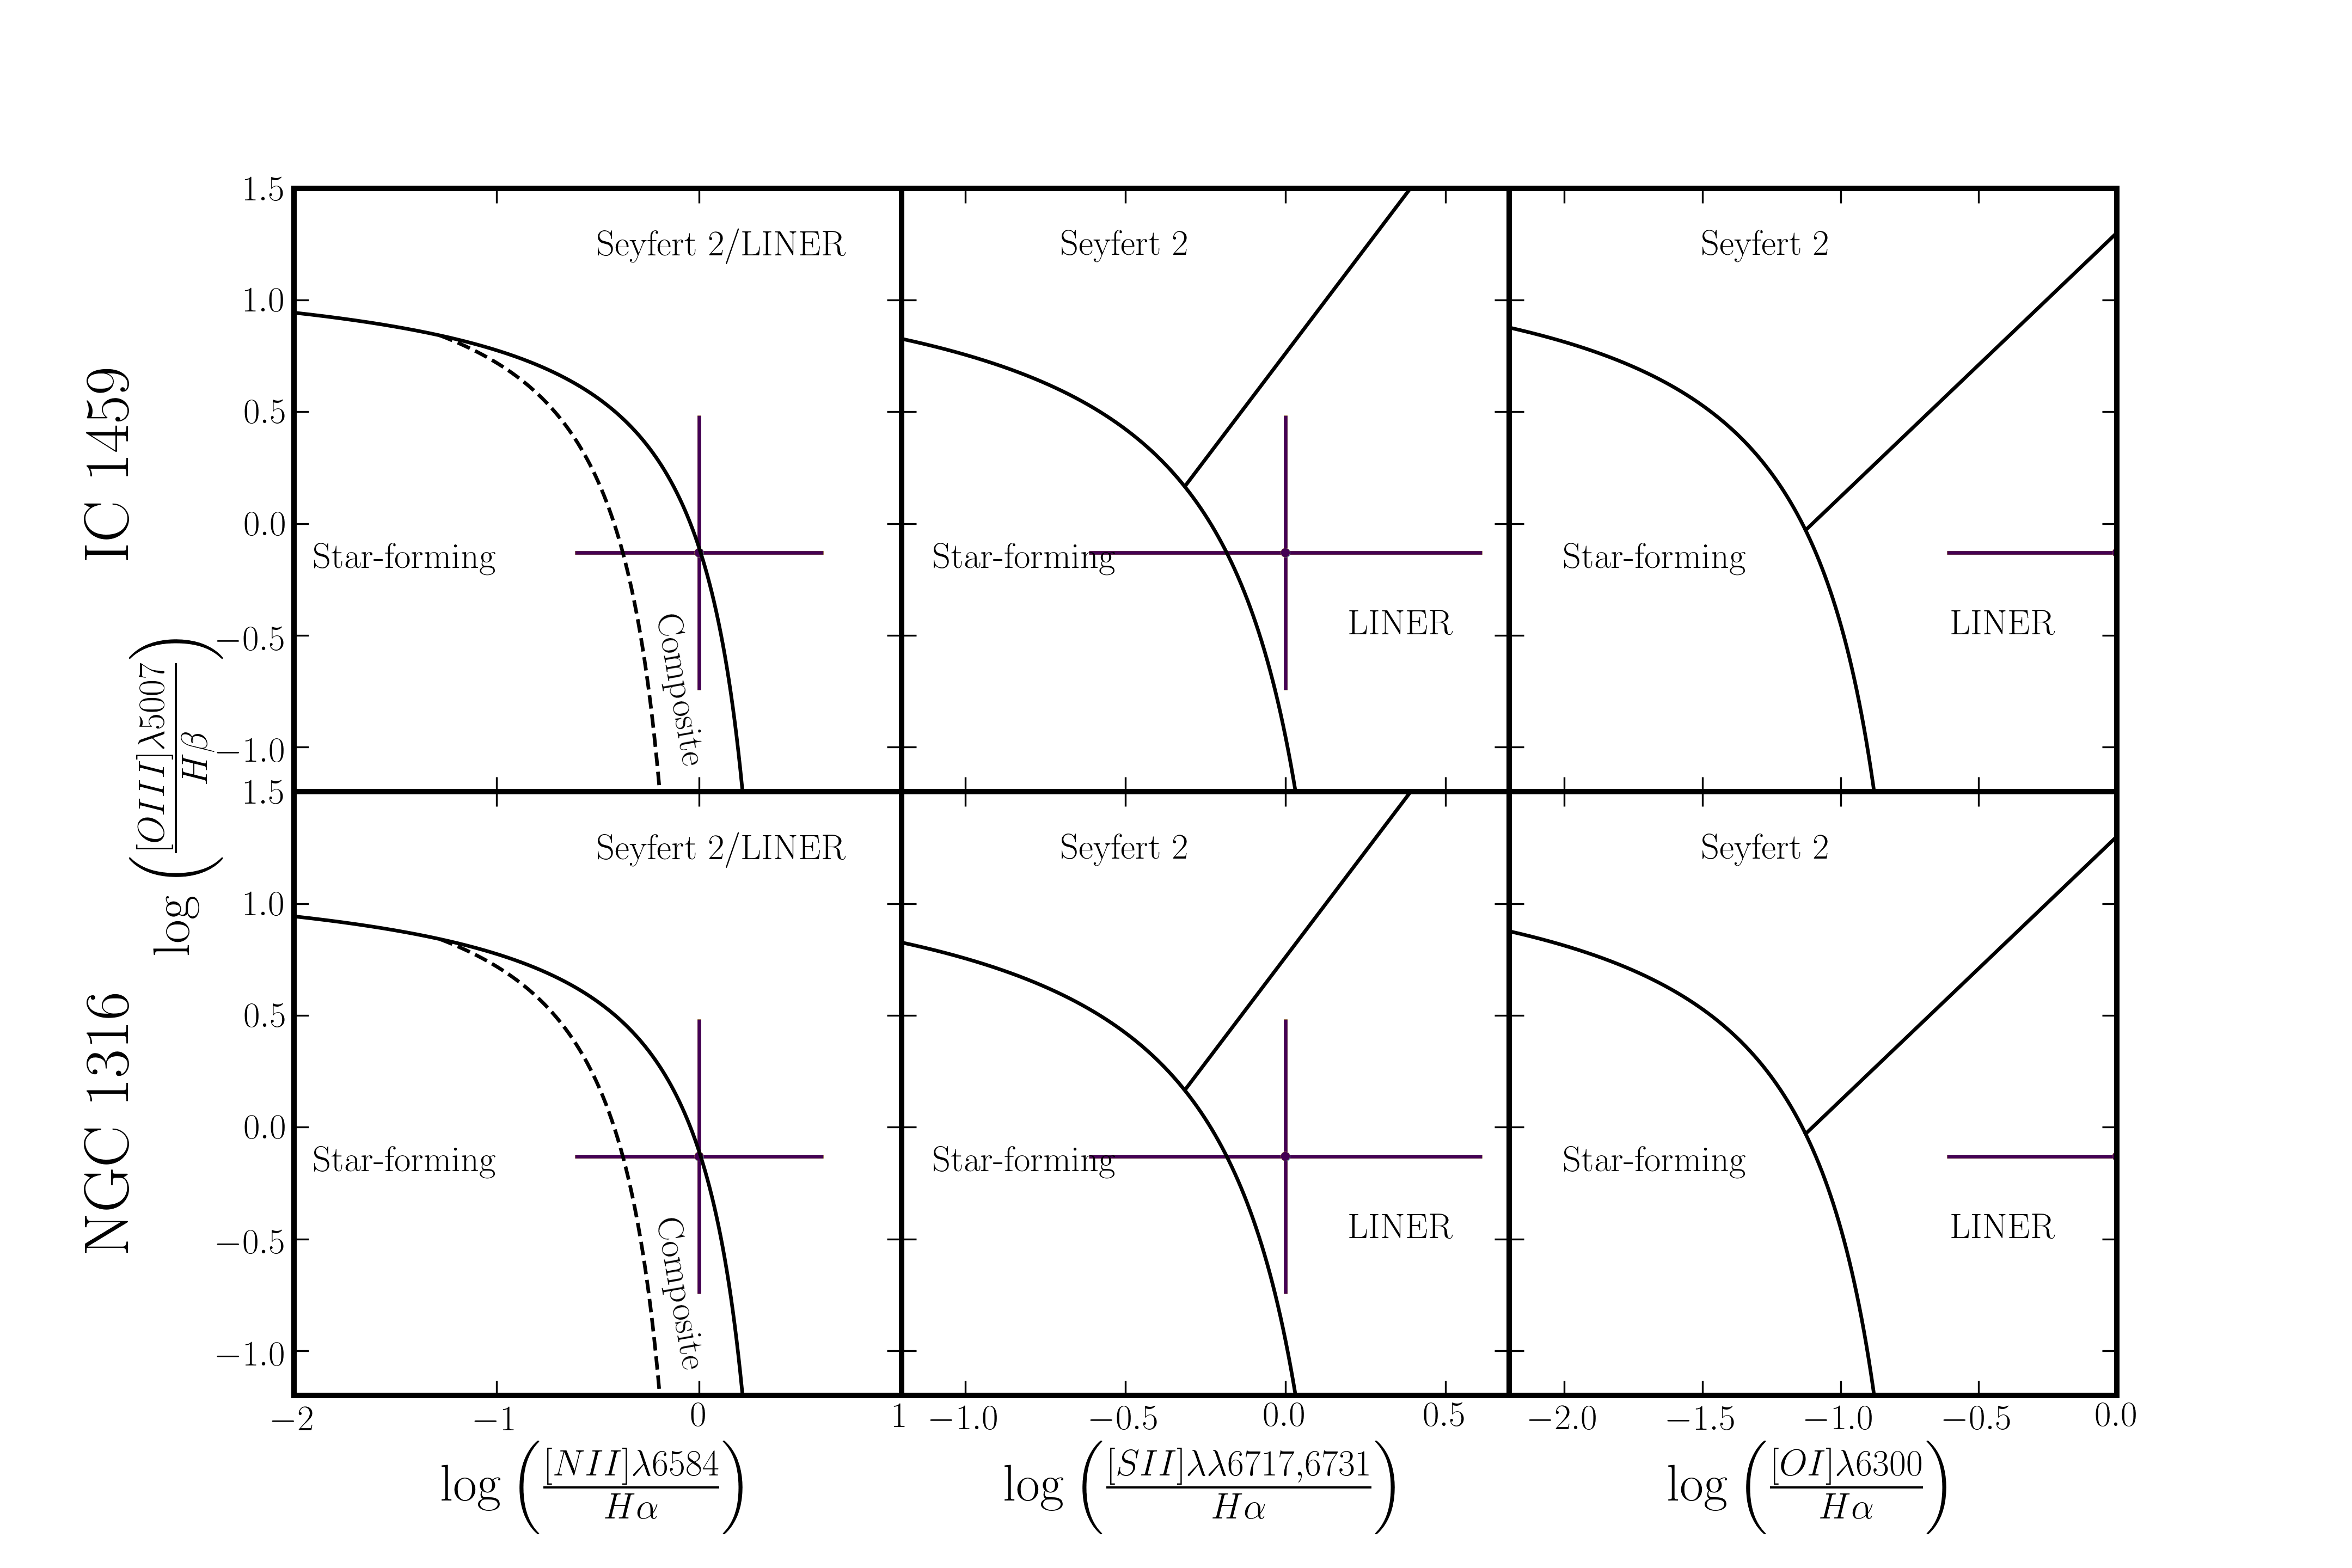
\includegraphics[width=.9\textwidth]{chapter5/BPT.png}
			\caption[BPT plots]{BPT plots for IC 1459 and NGC 1316. The colour scale (blue to yellow) represents increasing distance from the galaxy centre. The classification boundaries are from \citet{Kewley2006}.\label{fig:BPT}}
		% \end{figure}

		% \begin{figure}
		% 	\centering
			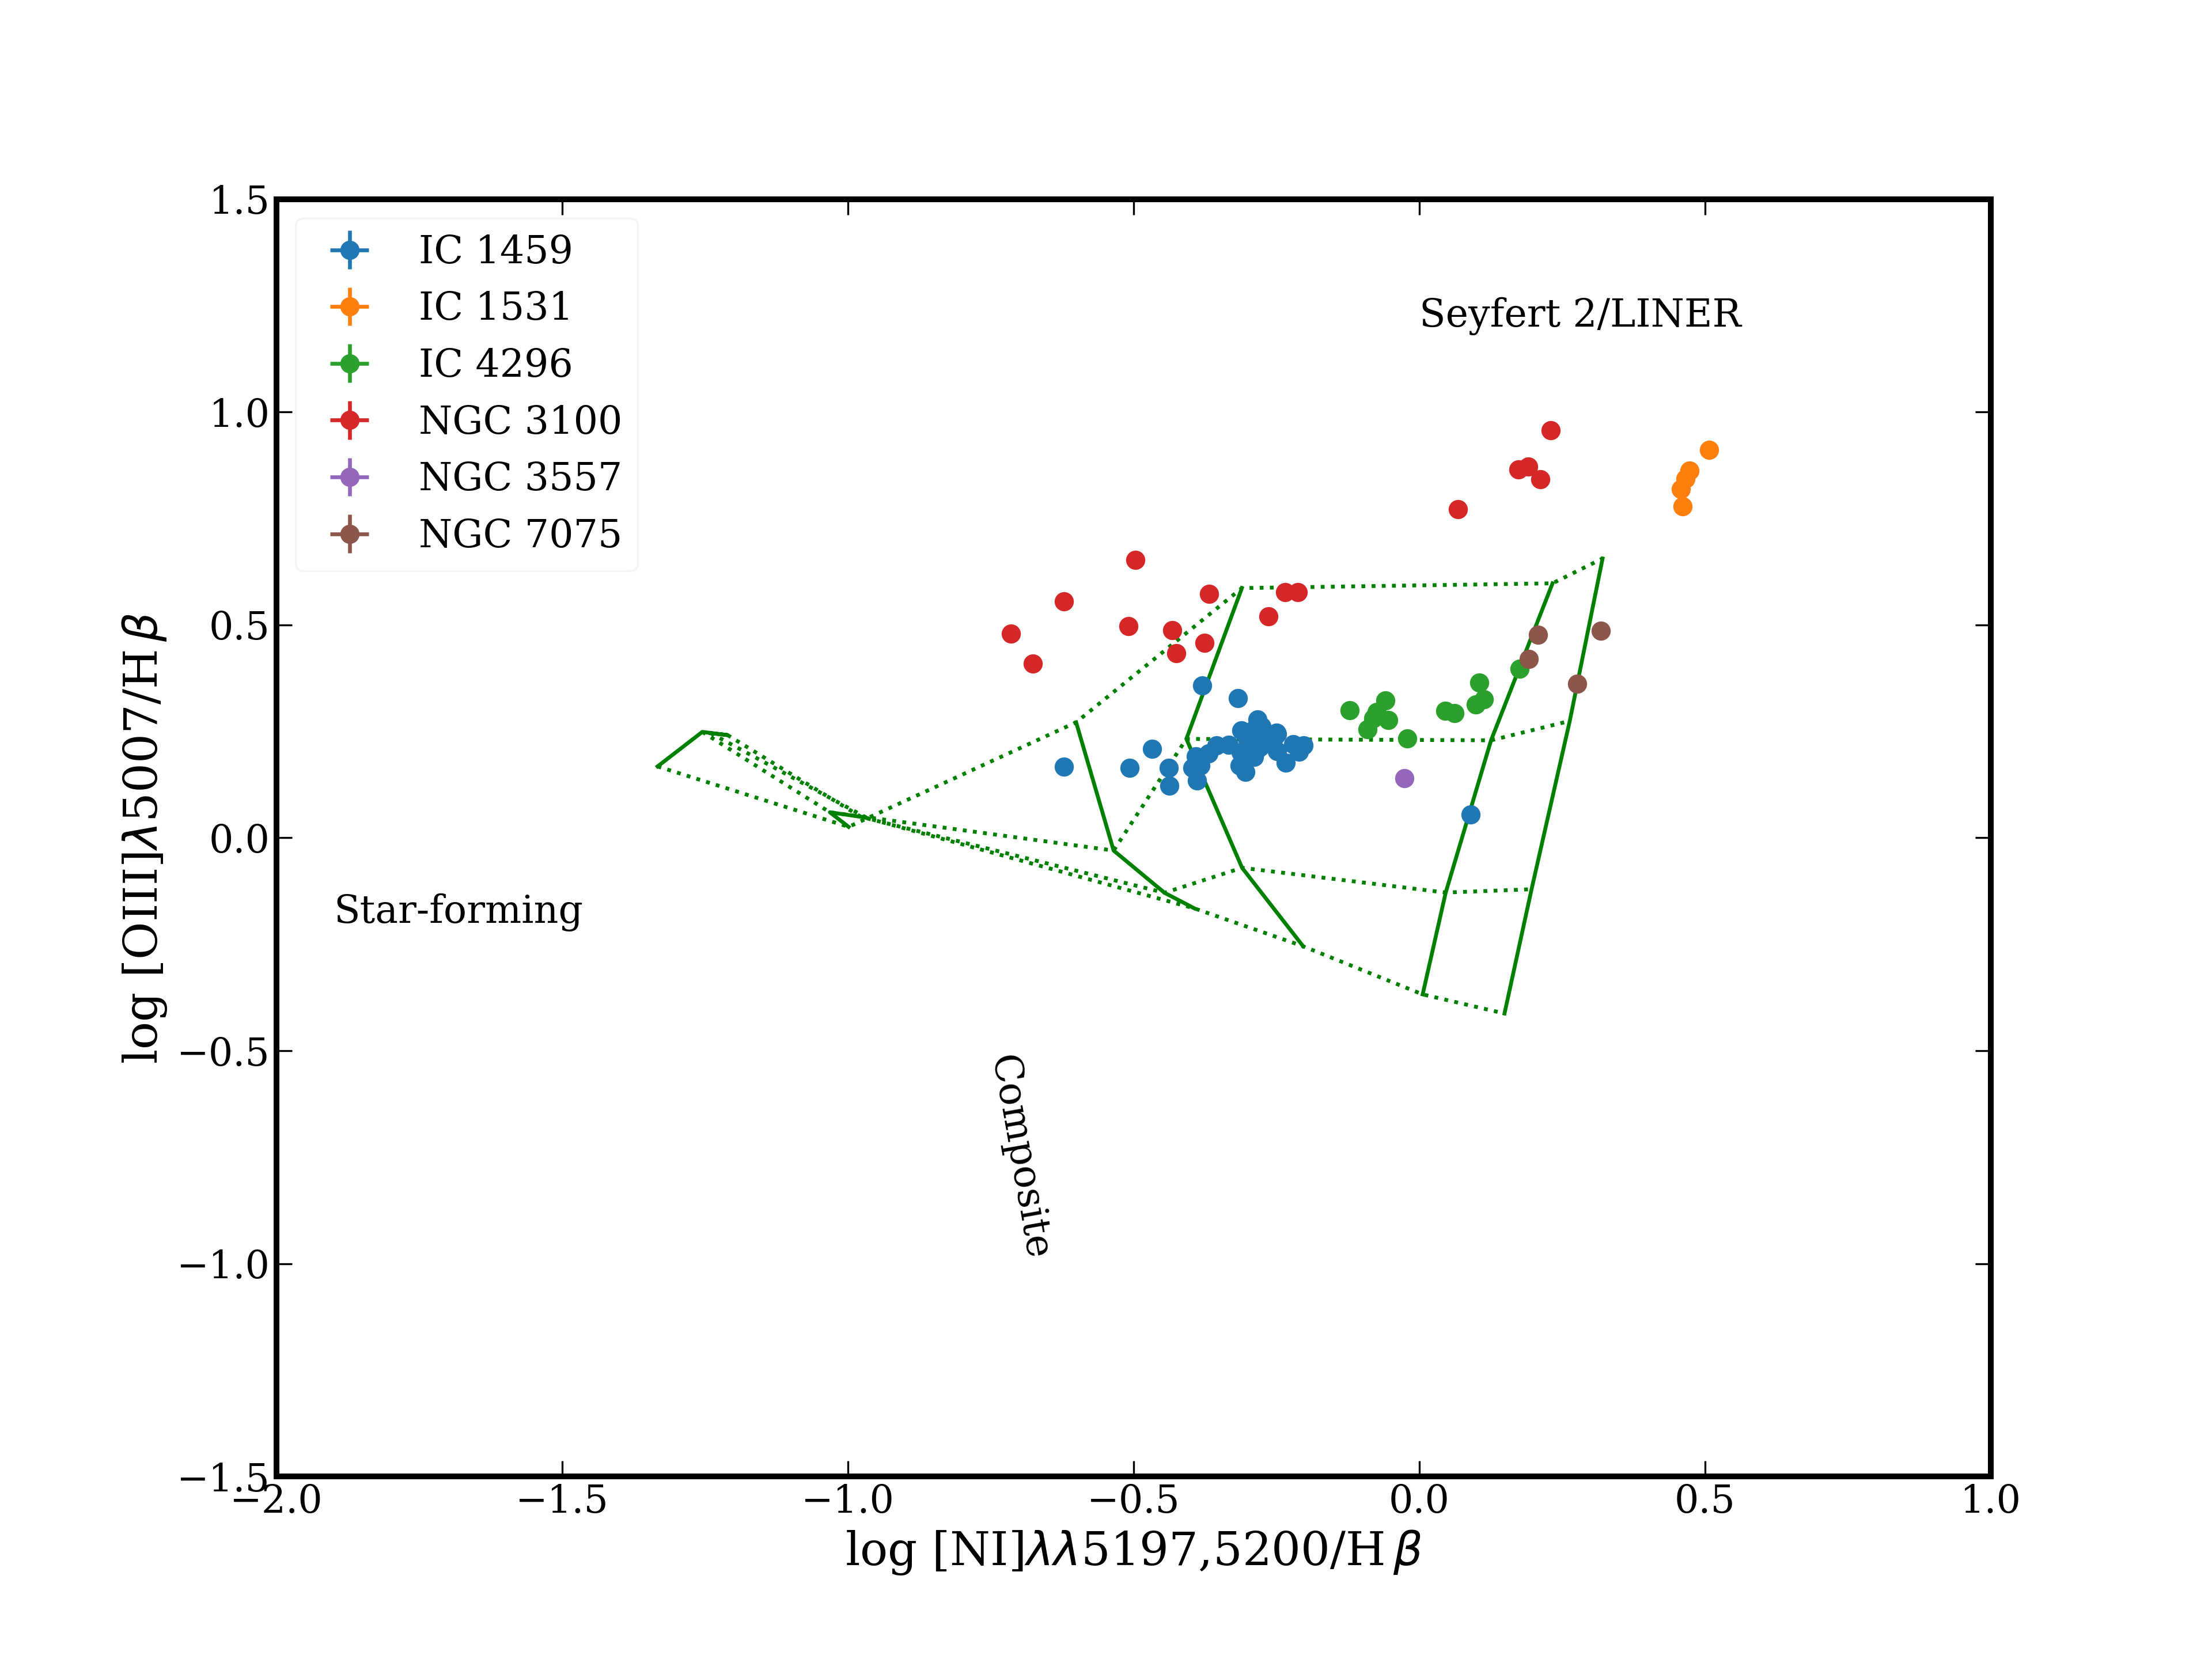
\includegraphics[width=0.7\textwidth]{chapter5/SAURON.png}
			\caption[An alternative diagnostic plot]{SAURON diagnostic plot for the line ratios available in the VIMOS datacubes. To show the expected position of LINERs on the SAURON plot, the MAPPINGS-III shock model grid of \citet{Allen2008} is shown in green. The solid lines are lines of constant shock velocity (from 150 to 1000\,$\mathrm{km\,s^{-1}}$) and the dotted lines are lines of constant magnetic parameter $b \equiv B/\sqrt{n}$ (from 0.5 to 4.0), where $B$ is the magnetic field strength and $N$ the (pre-shock) particle number density \citep{Dopita1996}. All models assume an electron density of $n_\mathrm{e} = 1\,\mathrm{cm^{-3}}$.\label{fig:SAURON}}
		\end{figure}
		\restoregeometry

		\begin{figure}
			\centering
			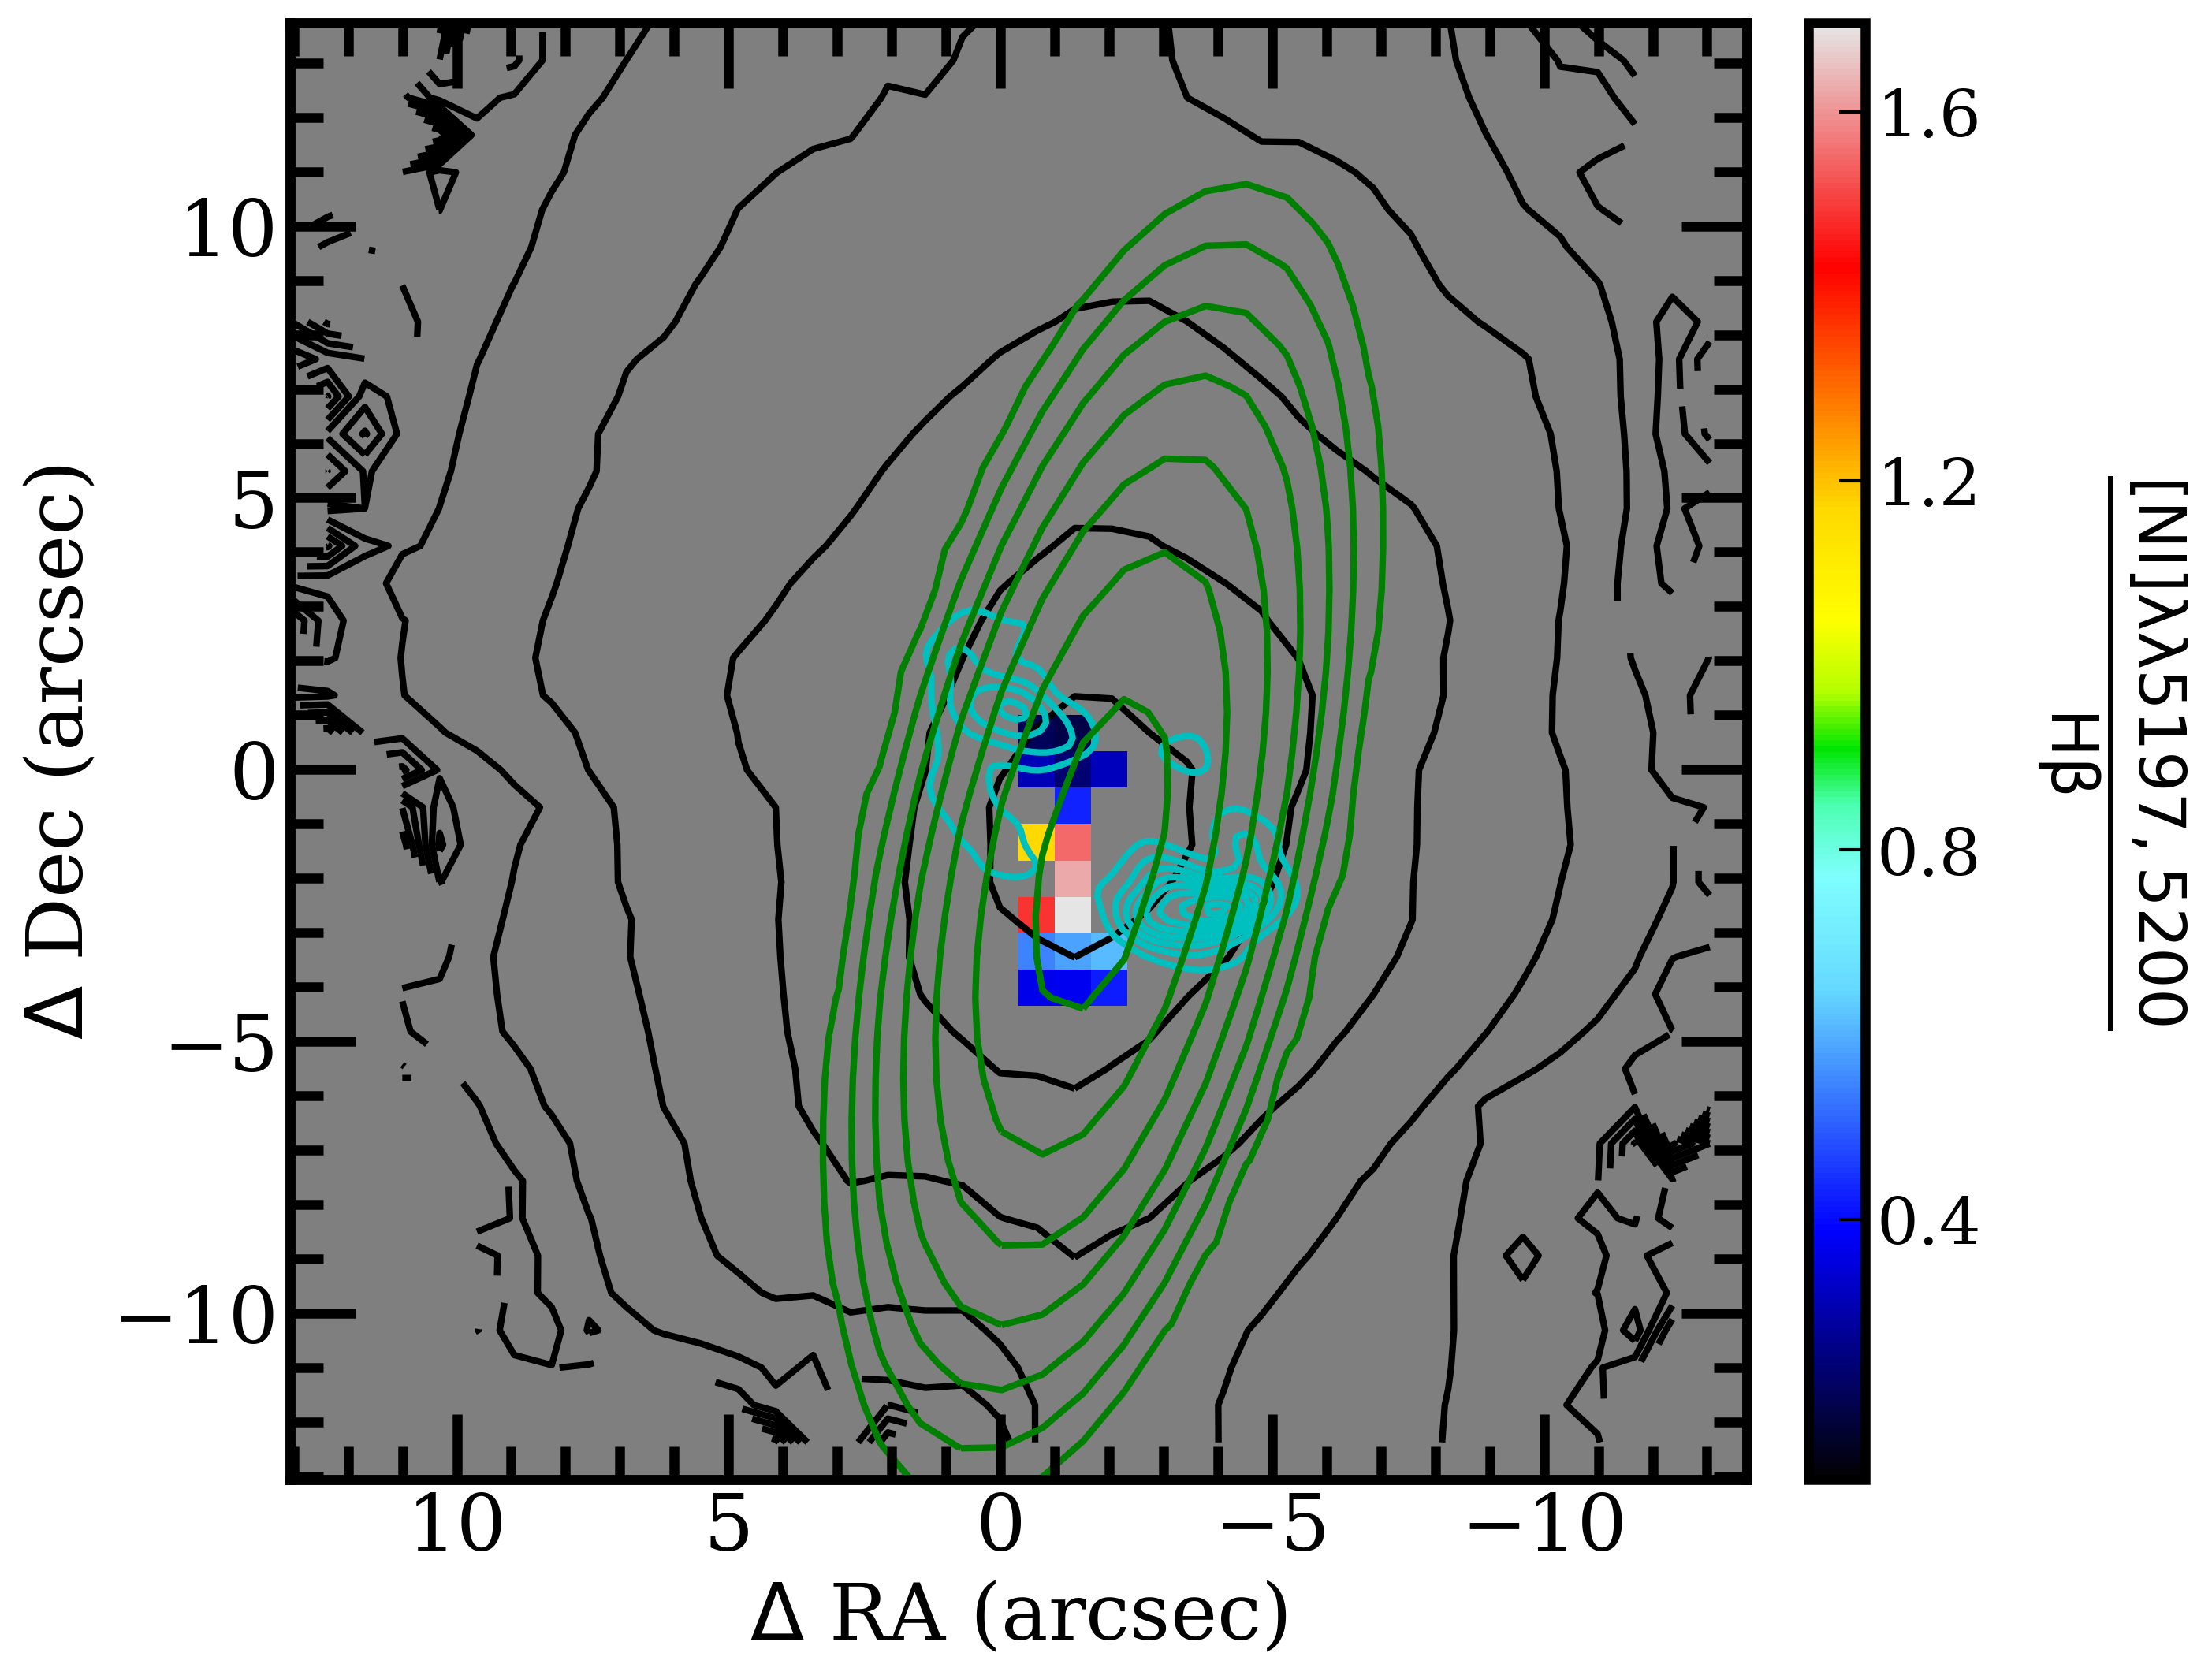
\includegraphics[width=0.5\textwidth]{chapter5/vimos/ngc3100_NI_Hb.png}
			\caption[NGC 3100 \bracket{\ion{N}{i}}/H$\beta$ line ratio map]{The [\ion{N}{i}]/H$\beta$ line ratio map of NGC 3100, showing the hardest ionization field is in gap in the CO ring (white contours), spatially coincident with the radio jet (green contours). Surface brightness contours are in black.}
			\label{fig:ngc3100_NI_Hb}
		\end{figure}
 
	\subsection{WHaN2 Plots}
		\label{subsec:WHaN2}
		\begin{figure}[t]
			\centering
			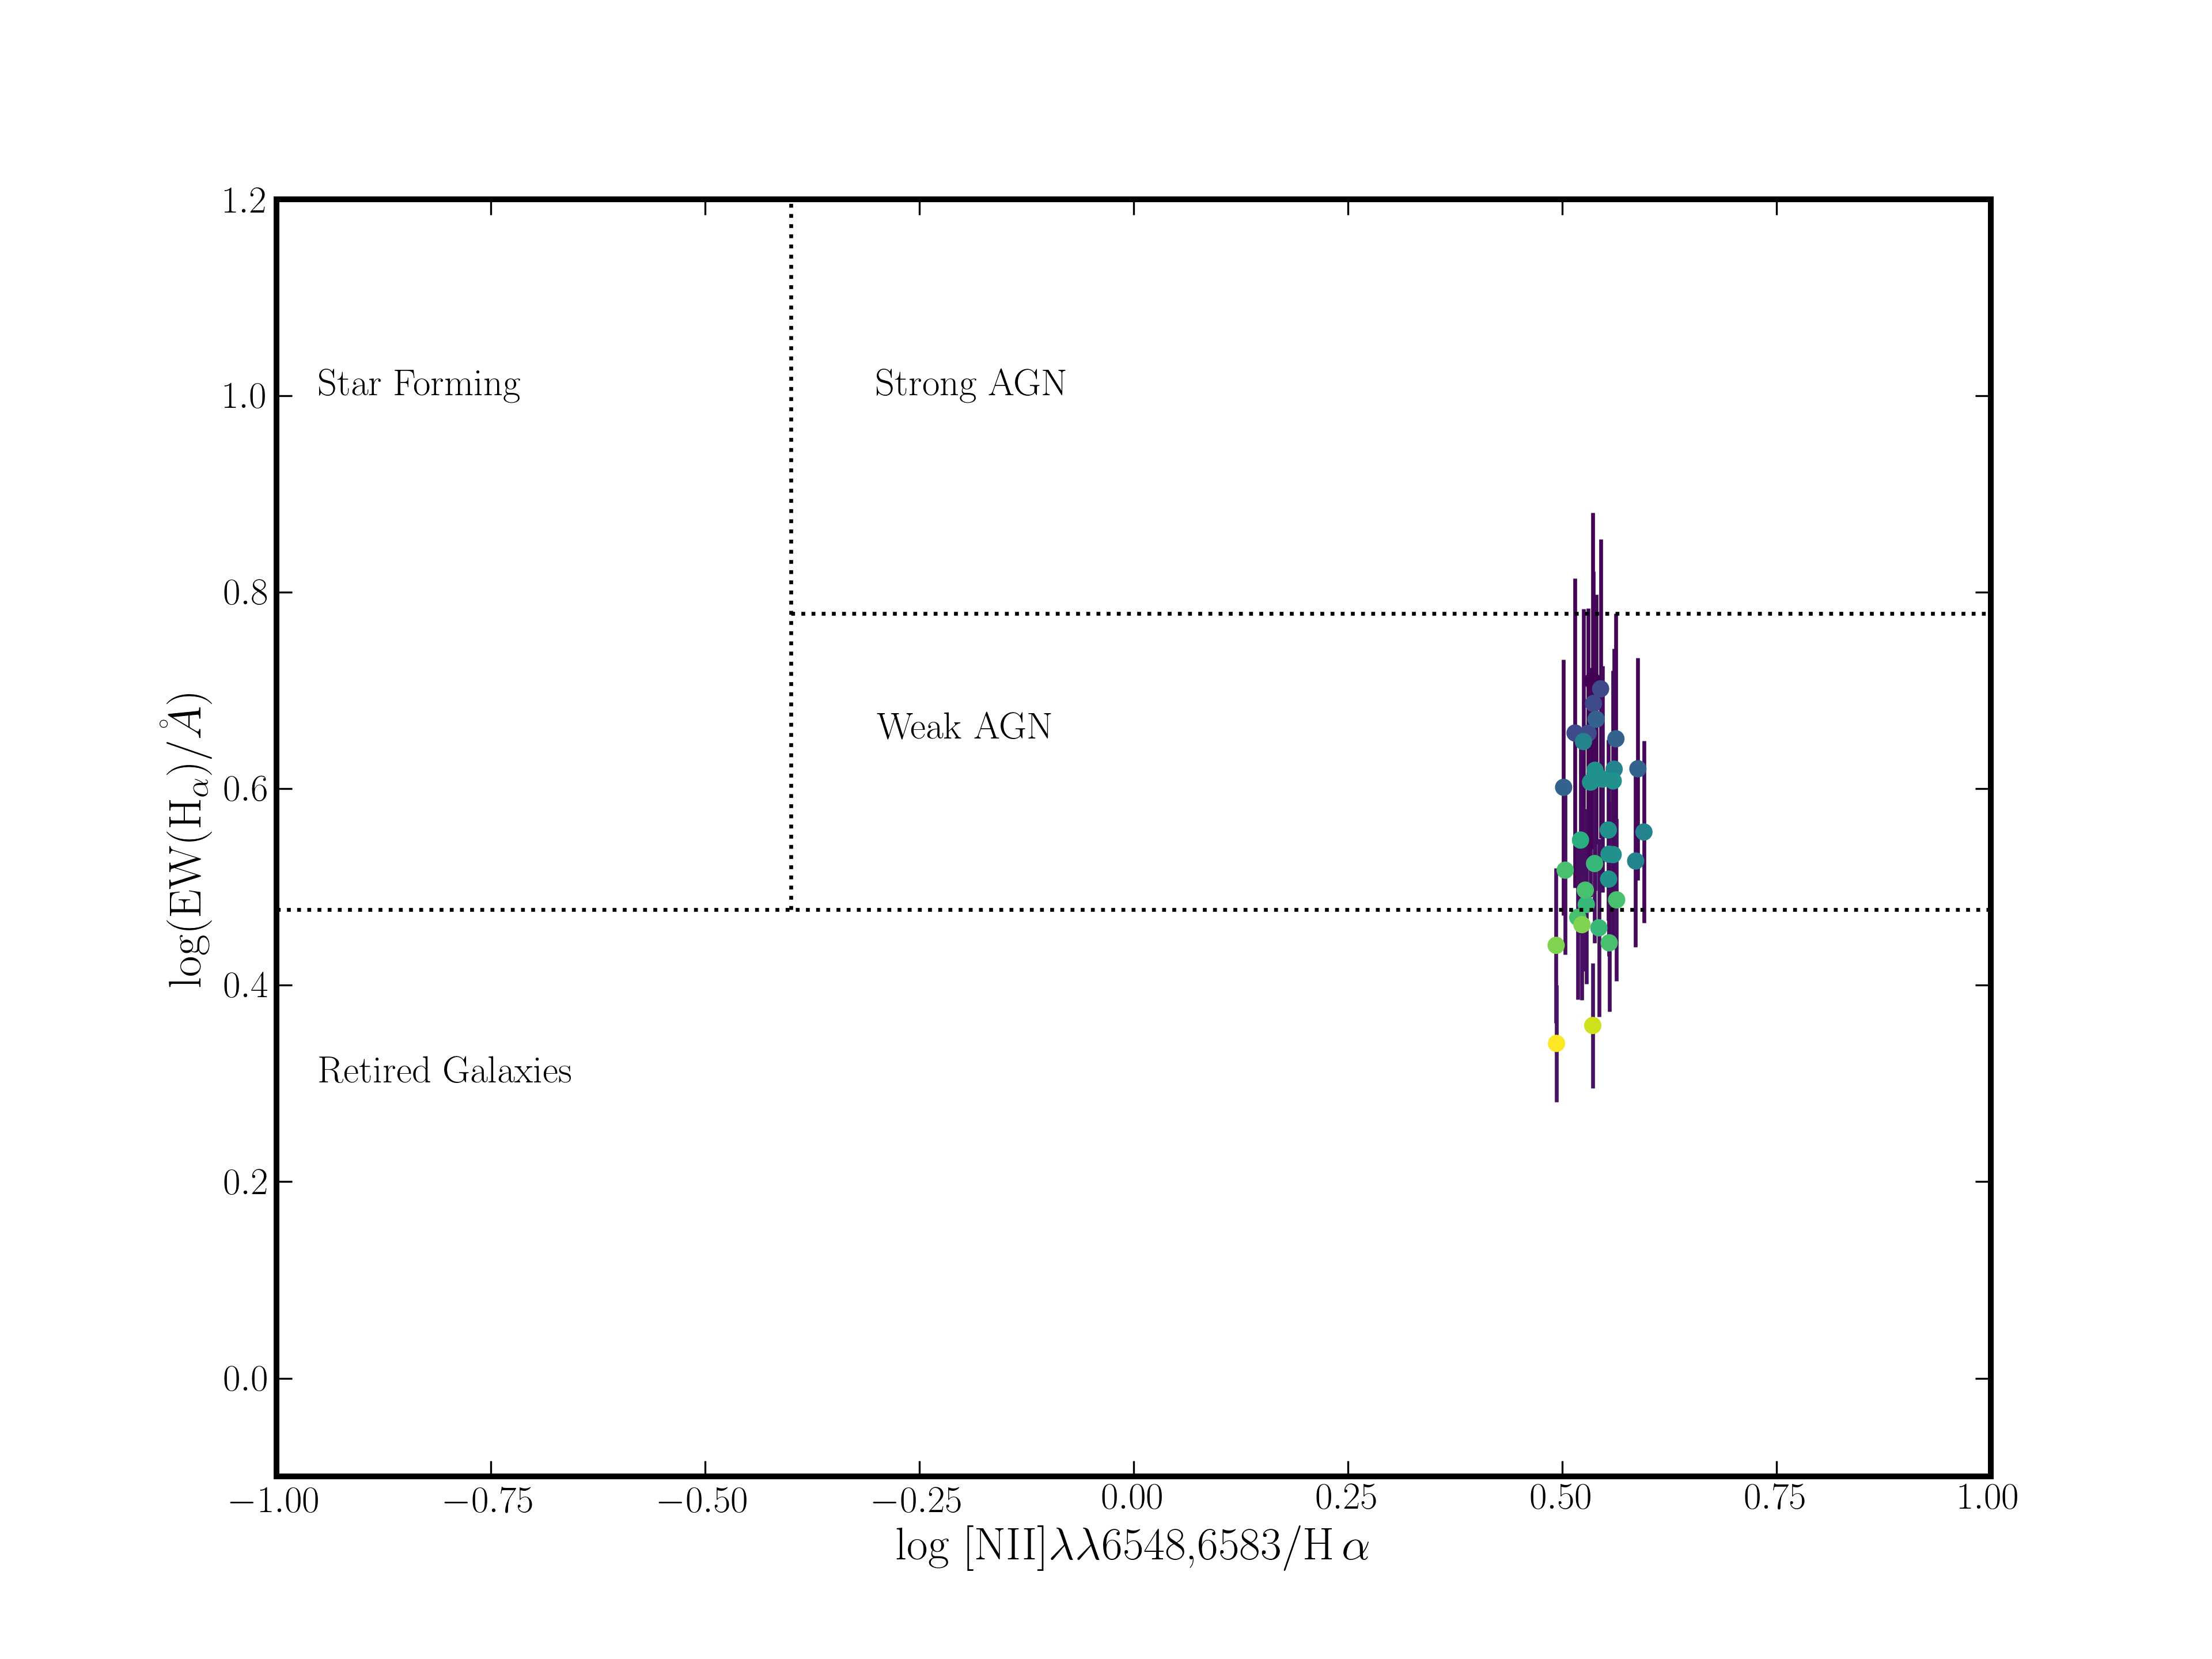
\includegraphics[height=.43\textheight]{chapter5/WHaN2.png}
			\caption[WHaN2 plot for IC 4296]{WHaN2 plot for IC 4296. The colour scale (blue to yellow) represents increasing distance from the galaxy centre.}
			\label{fig:WHaN2}
		% \end{figure}

		% \begin{figure}
		% 	\centering
			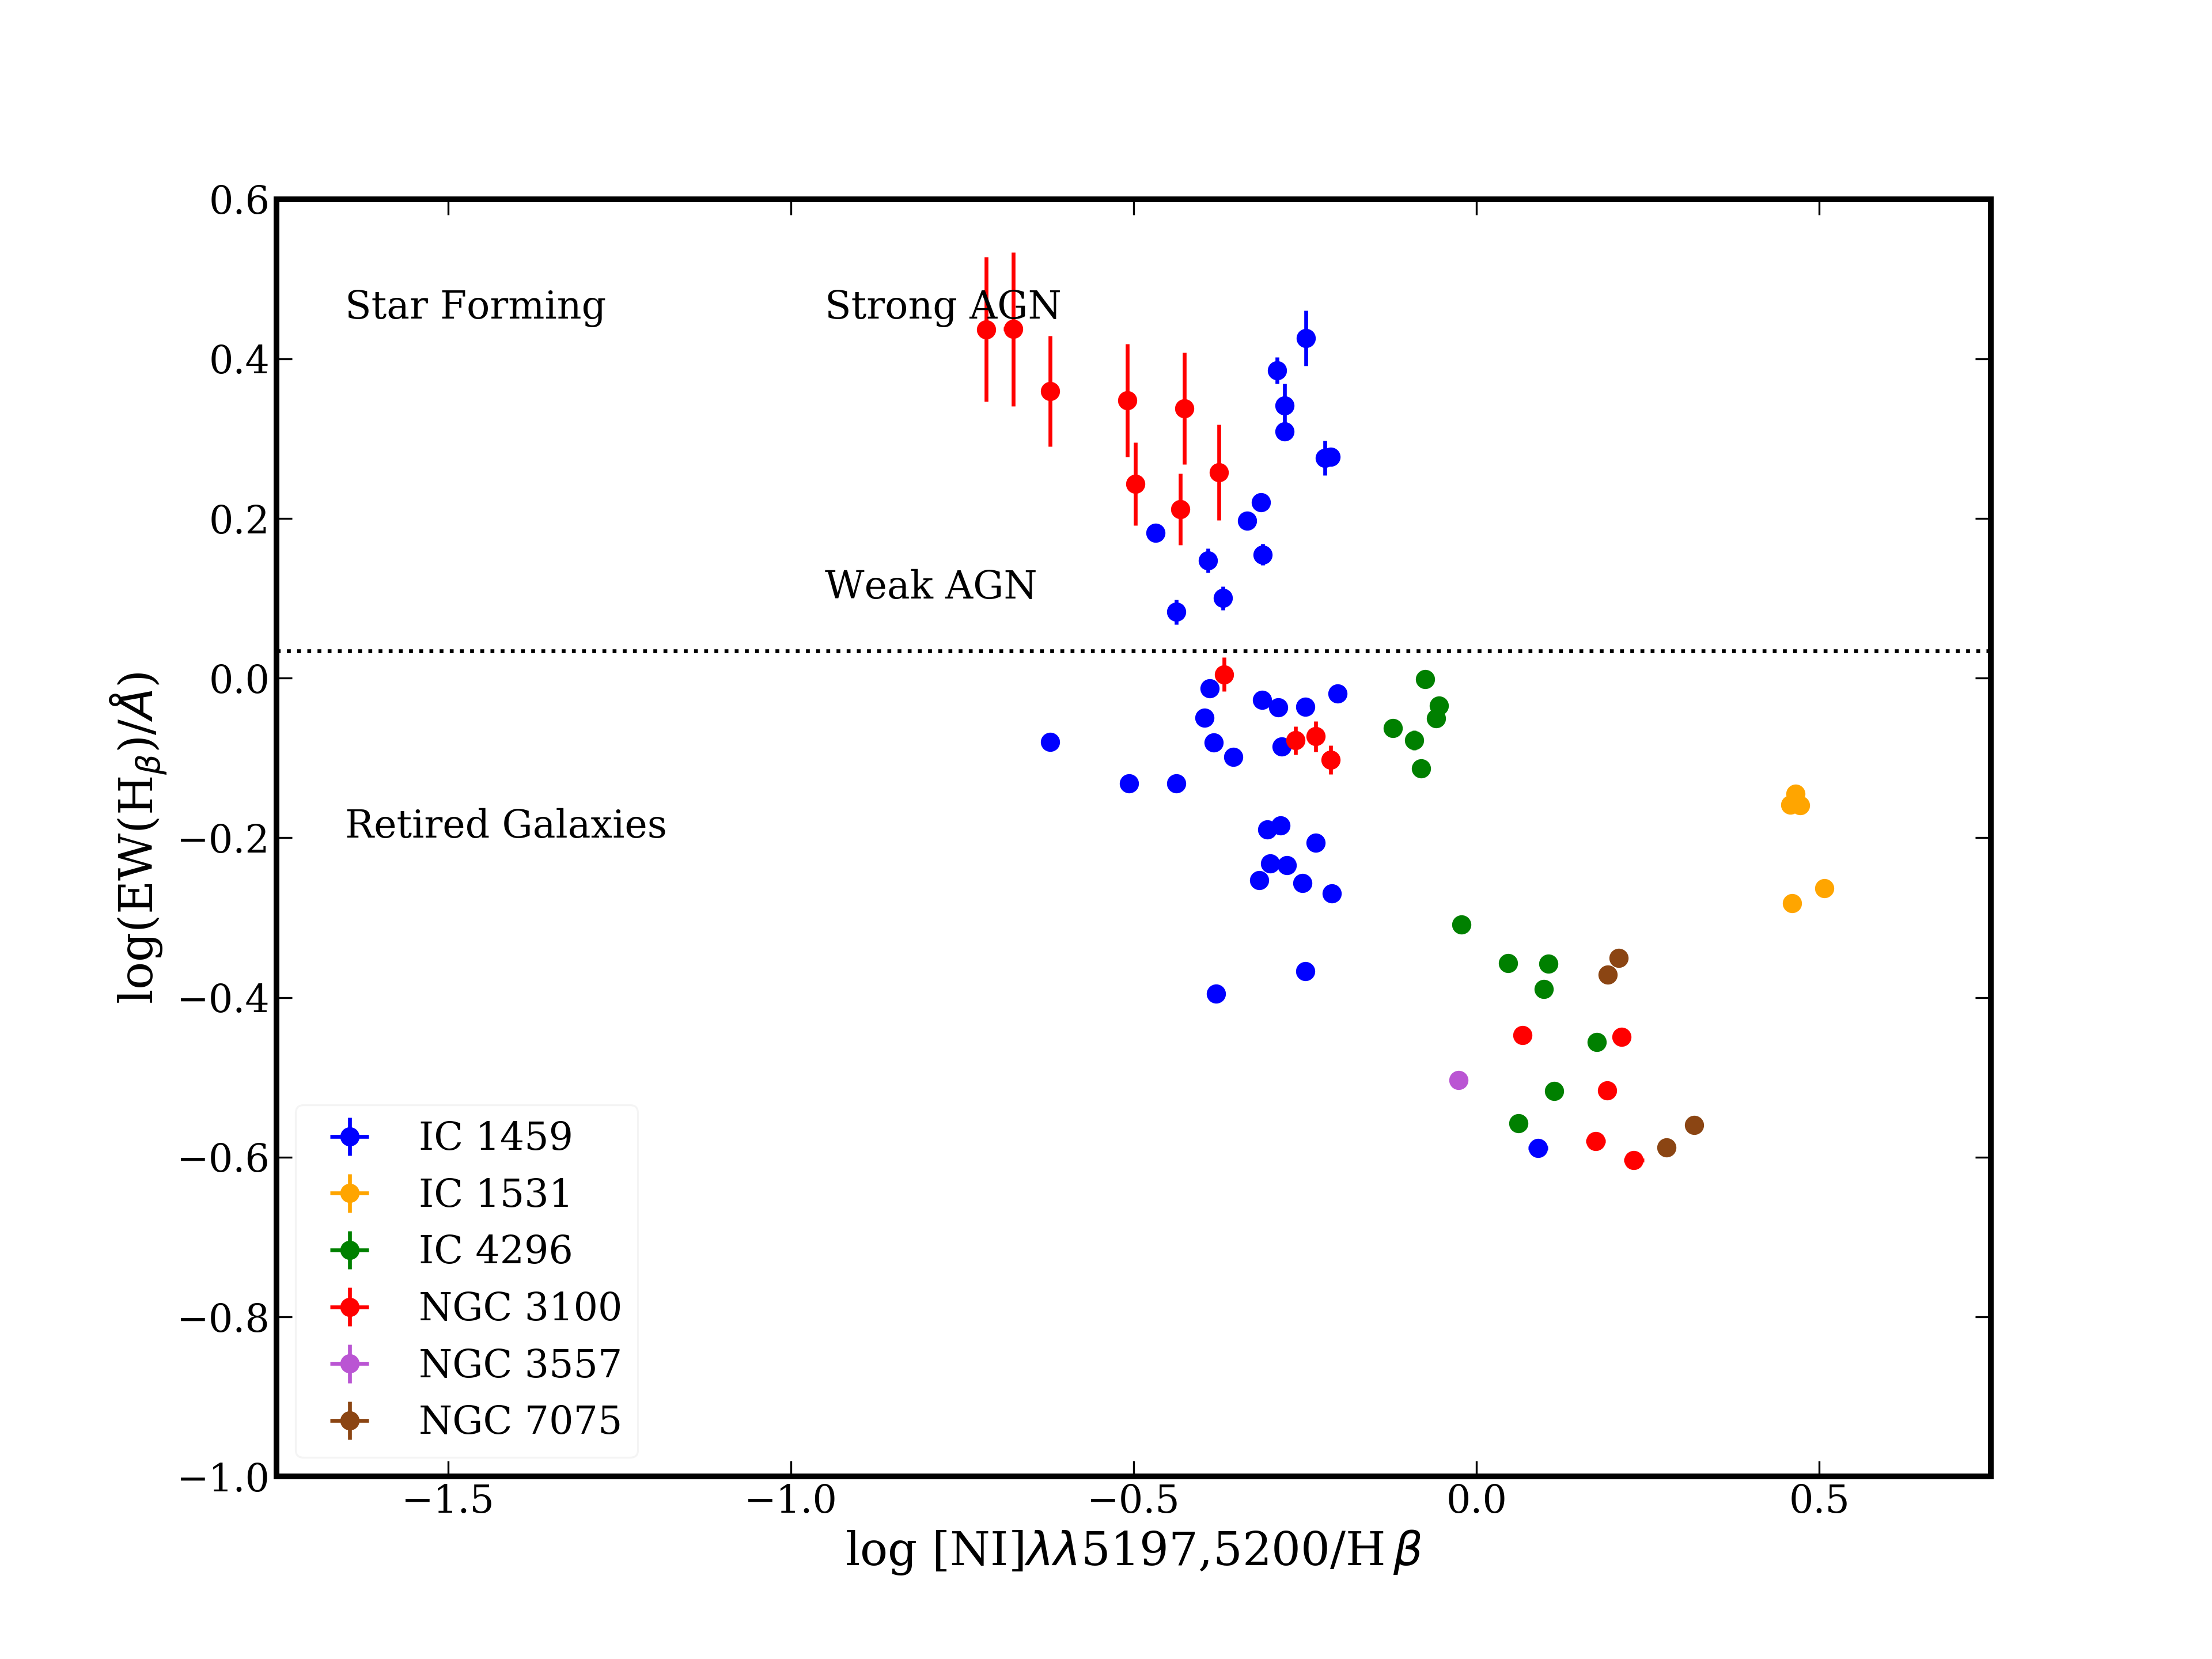
\includegraphics[height=.43\textheight]{chapter5/WHbN1.png}
			\caption[VIMOS WHbN1 plot]{VIMOS WHbN1 plot. All galaxies have decreasing H$\beta$ emission with increasing distance from the galaxy centre.}
			\label{fig:WHbN1}
		\end{figure}

		The final spatially-resolved line ratio diagnostic plot that we use is that of the equivalent width of H$\alpha$ versus $\log([\text{\ion{N}{ii}}]/H\alpha)$, known as the WHaN2 plot \citep{CidFernandes2011}. We interpret the strong AGN, weak AGN and retired regions on this plot as Seyfert 2, LINER-AGN and LIER classifications, respectively. Passive (i.e.\ line-less) galaxies are marked with crosses instead of circles. Fig.\,\ref{fig:WHaN2} shows the WHaN2 plot for the MUSE derived emission lines of IC 4296 where almost all the bins fall within the weak AGN (LINER-AGN) class. This is consistent with the measurements from the VIMOS observations of the IC 4296 as shown in the SAURON diagnostic plot, where IC 4296 is well within the shocks grid (i.e.\ LINERs; see Fig.\ \ref{fig:SAURON}). We do not include IC 1459 and NGC 1316, as they have already been classified via the classic BPT plots (see Section \ref{subsec:BPT}). 

		For the emission lines measured from the VIMOS datacubes, we use H$\beta$ as a proxy for H$\alpha$ and [\ion{N}{i}] as a proxy for [\ion{N}{ii}] utilising the relations found in Section \ref{subsec:Ndec} to transform the classification boundaries (see Section \ref{subsec:Ndec}). We call the resulting diagnostic plot the WHbN1 plot, shown in Fig.\,\ref{fig:WHbN1}. While in Section \ref{subsec:BPT} (Fig.\,\ref{fig:SAURON}) we showed that most of these galaxies had line ratios consistent with being ionized by shocks such as in LINER-like galaxies, Fig.\,\ref{fig:WHbN1} shows that for IC 1459 and NGC 3100, the ionizing photons originate from the AGN. 

		\FloatBarrier
	
		\begin{figure}
			\centering
			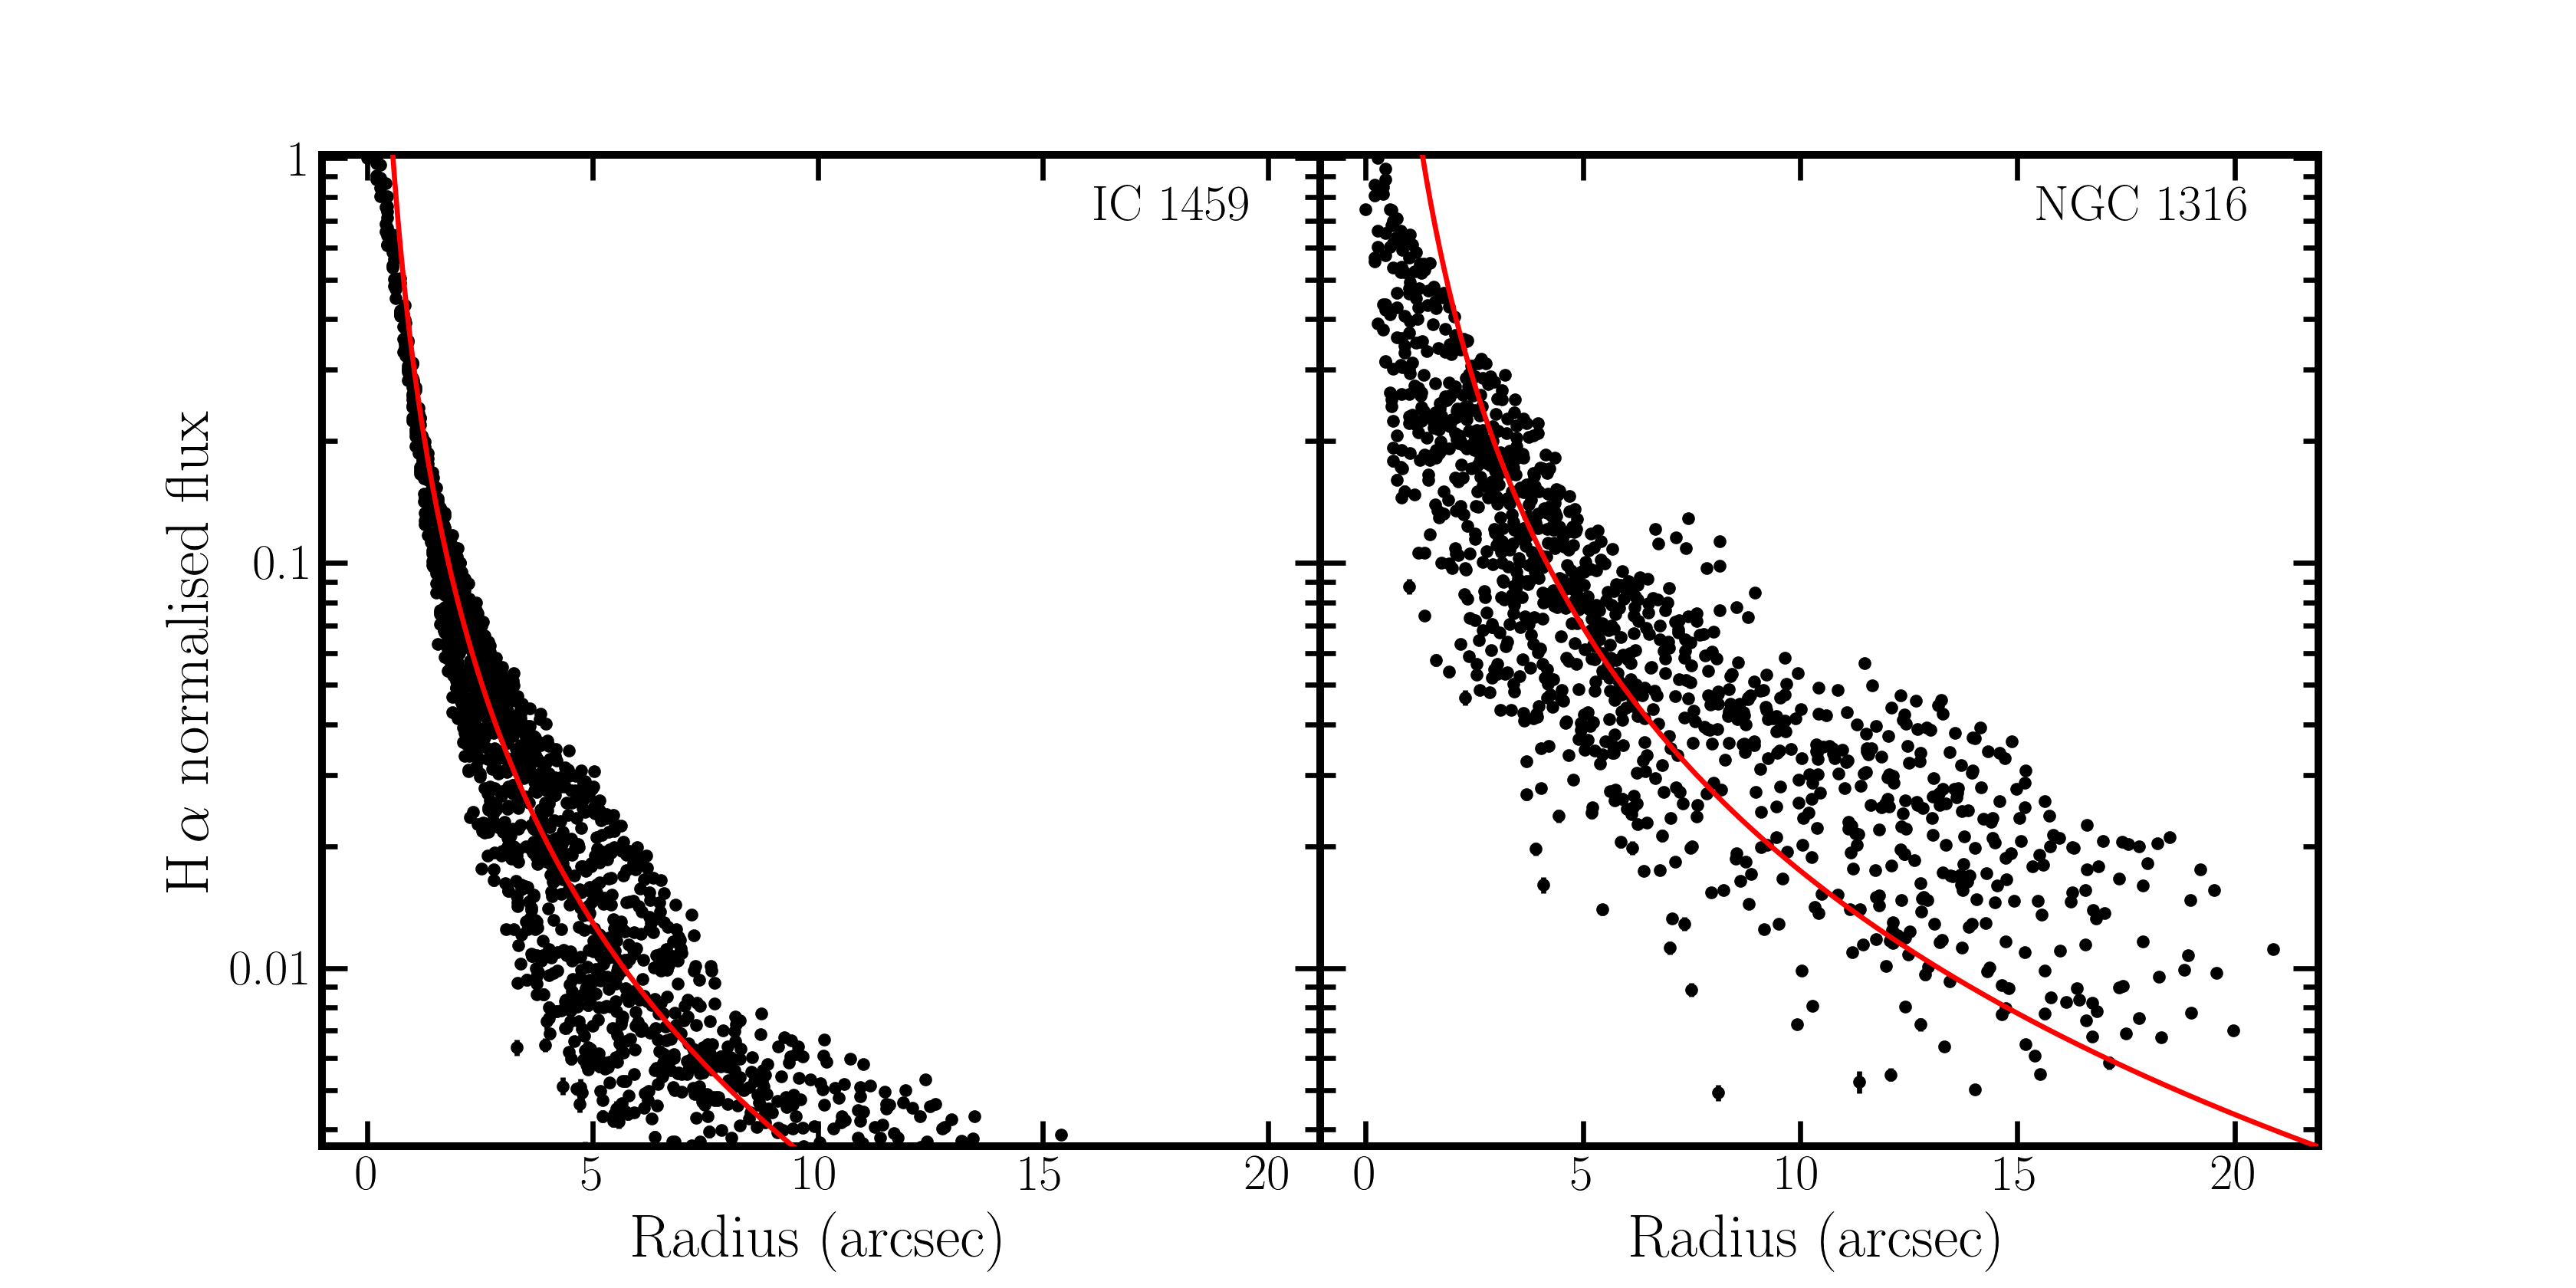
\includegraphics[width=0.73\textwidth]{chapter5/muse/Halpha_profile.png}
			\caption[MUSE H$\alpha$ radial profiles]{H$\alpha$ flux radial profiles derived from the MUSE datacubes. Solid red lines show $F(\mathrm{H\alpha}) \propto r^{-2}$ convolved with a Gaussian function of width equal to the mean seeing taken from the fits file headers. This accounts for the point-spread function (PSF) of the observations.\label{fig:Ha_profile_MUSE}} 
		% \end{figure}

		% \begin{figure}
		% 	\centering
			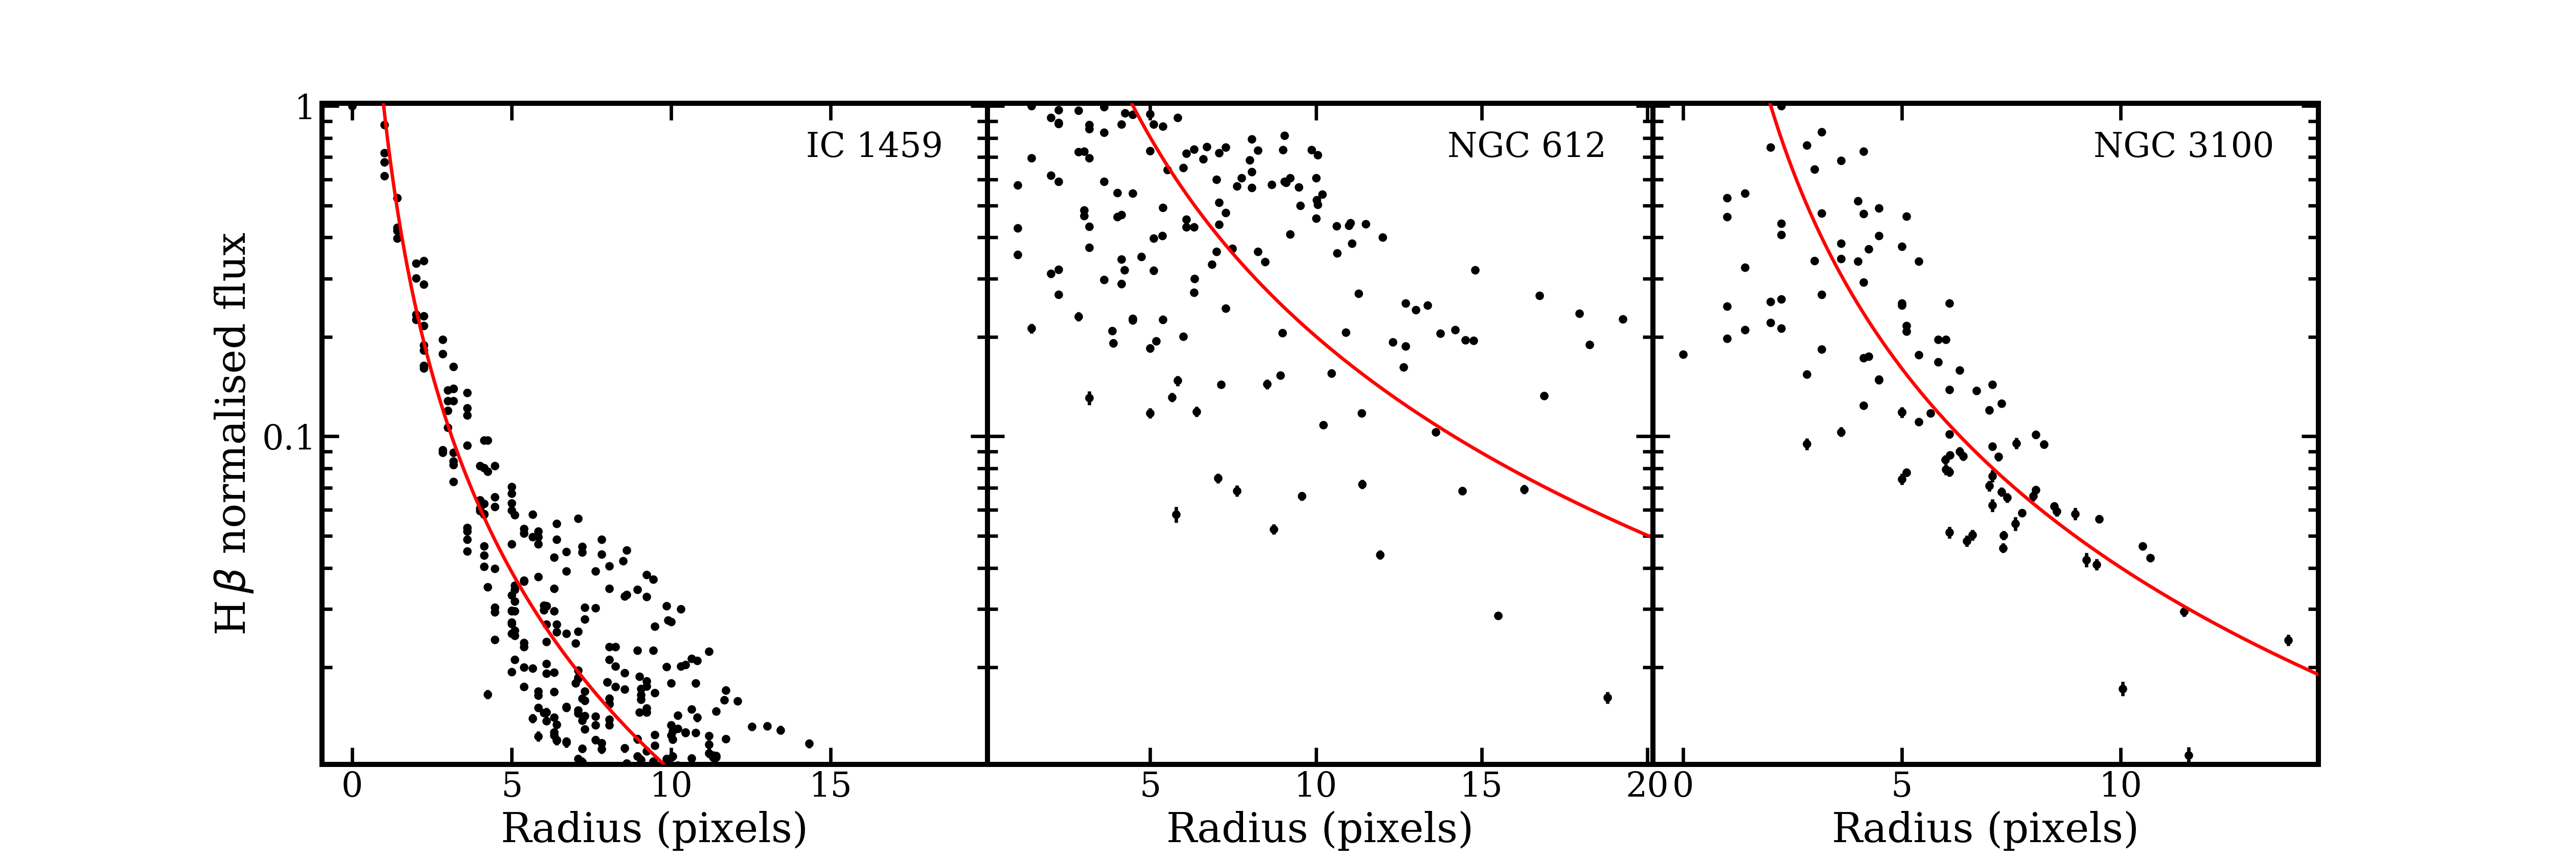
\includegraphics[width=1.1\textwidth]{chapter5/vimos/Hbeta_profile.png}
			\caption[VIMOS H$\beta$ radial profiles]{H$\beta$ flux radial profiles derived from the VIMOS datacubes. Solid red lines show $F(\mathrm{H\beta}) \propto r^{-2}$ convolved with a Gaussian function of width equal to the mean seeing (see Table \ref{tab:observations}). This accounts for the PSF of the observations. \label{fig:Hb_profile_VIMOS}} 
		\end{figure}

		\FloatBarrier
	
	\subsection{H$\beta$ Profiles}
		\label{subsec:Hb}
	
		As discussed in Section \ref{sec:ETG}, many galaxies classified as LINERs are in fact LIERs \citep[see e.g.][]{Sarzi2005, Sarzi2010, Singh2013, Belfiore2016}, i.e.\ the source of the ionizing radiation is not concentrated in the nuclear regions of the galaxies. As we can see from Figs.\ref{fig:BPT} and \ref{fig:SAURON}, most bins of a given galaxy are tightly grouped together on the BPT plots. To check if the ionizing radiation is entirely due to an AGN throughout the host galaxy, we plot the H$\alpha$ and H$\beta$ flux radial profiles for the MUSE and VIMOS data in Figs.\,\ref{fig:Ha_profile_MUSE} and \ref{fig:Hb_profile_VIMOS}, respectively. A point source, such as an AGN, will result in a profile having a $r^{-2}$ shape, where $r$ is the distance of the bin from the galaxy centre. A shallower profile points to a spatially-extended source, presumably non-circumnuclear stellar processes such as star formation or radiation from pAGB stars (see Section \ref{subsubsec:JetFeedback}), as the dominant cause of the ionization in the outer parts of the galaxy (i.e.\ LIER rather than LINER). All the galaxies with spatially-extended Balmer emission in our Southern Sample revel a central point source as the dominant source of the ionizing photons. The H$\beta$ profile of NGC 612 has a larger scatter suggesting that stellar processes also have some impact (likely radiation from pAGB stars, as these galaxies are ETGs and therefore likely have low star-formation rates).

		


	\subsection{MEx Diagnostic Plots}
		\label{subsec:MEx}
		\begin{figure}[t!]
			\centering
			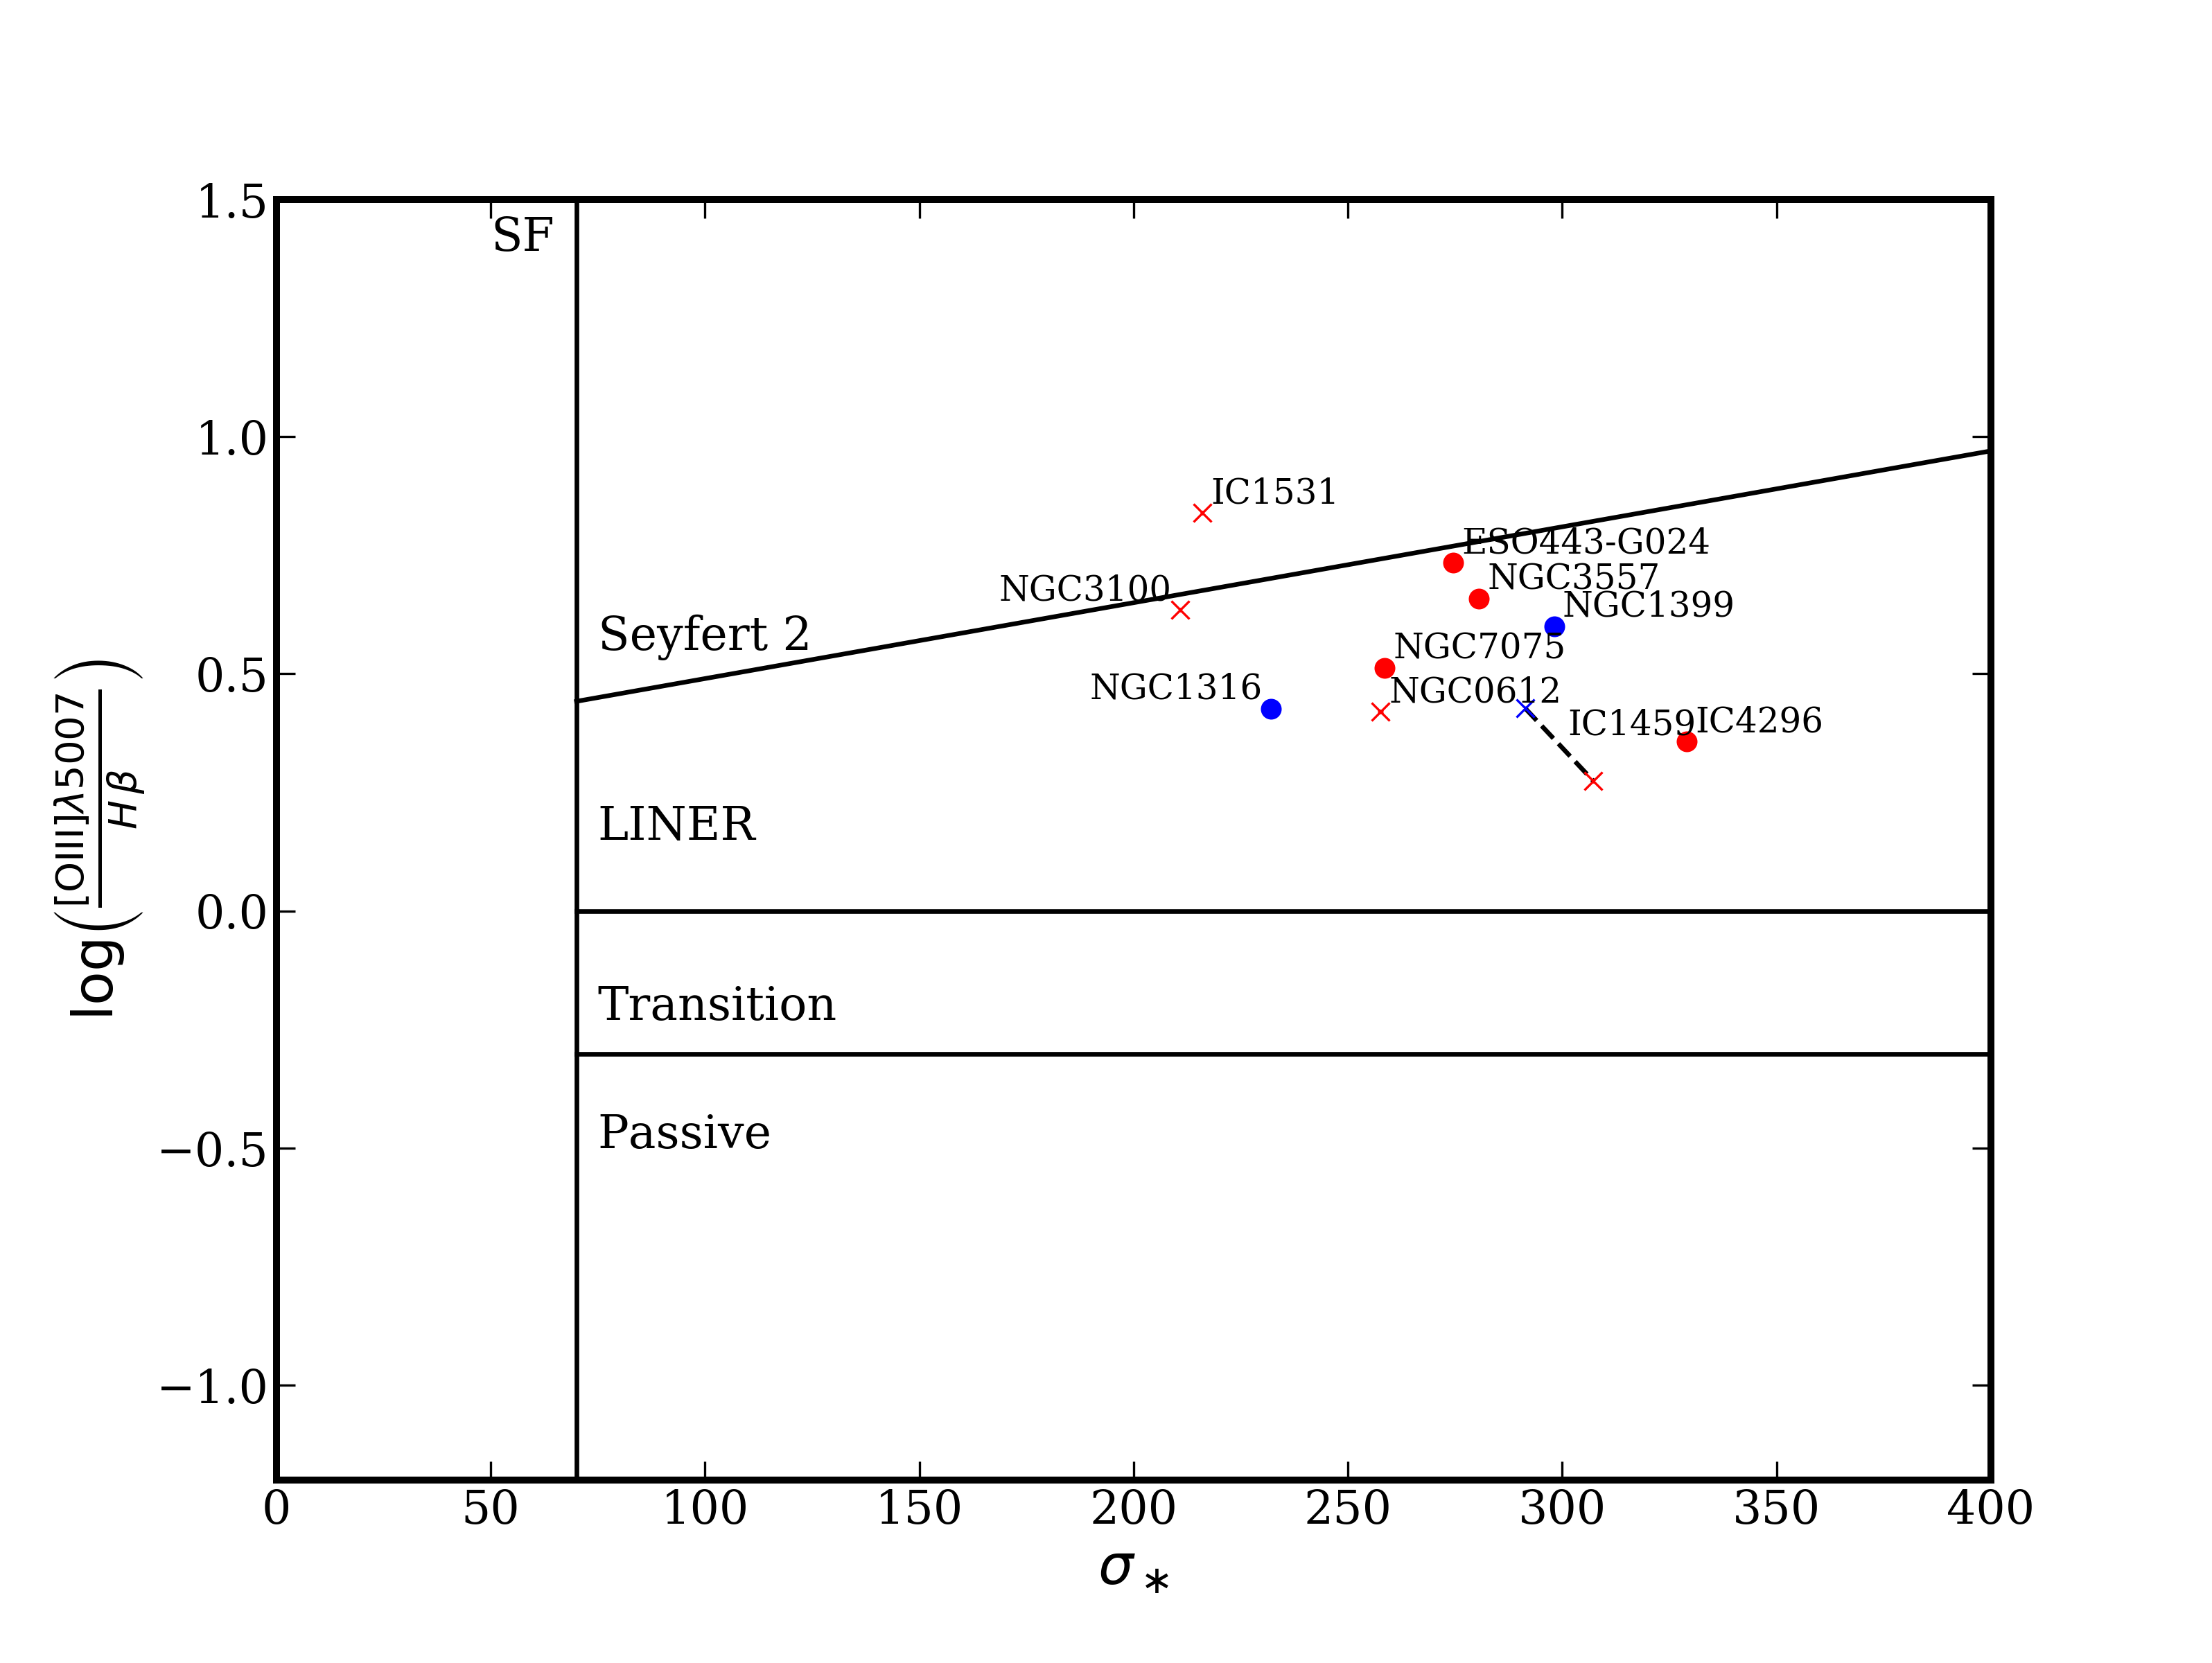
\includegraphics[width=\textwidth]{chapter5/nuclear_MEx.png}
			\caption[Nuclear mass\,--\,excitation plot]{Nuclear MEx plot, allowing to classify the sources of the ionizing radiation within the central 3\arcsec. Data points derived from the VIMOS and MUSE datacubes are in red and blue, respectively. Crosses mark galaxies with [\ion{O}{iii}]$\lambda$5007 equivalent width $> 0.8$\,\AA, while filled circles show galaxies with [\ion{O}{iii}]$\lambda$5007 equivalent width $\leqslant 0.8$\,\AA. The VIMOS and MUSE data points of IC 1459 are linked with a black dashed line. Classification boundaries are from \citet{Nyland2016}.}
			\label{fig:MEx}
		\end{figure}

		The mass\,--\,excitation (MEx) plot of \citet{Juneau2011} is useful to classify galaxies with intermediate excitation levels ($0.5 < \mathrm{[\ion{O}{iii}]/H\beta} < 8.0$), particularly as it does not depend on faint lines such as the [\ion{N}{I}] doublet. We use here the calibrations by \citet{Nyland2016}, including an attempt to separate LINERs powered by AGN from those powered by pAGB stars (the former have [\ion{O}{iii}] equivalent widths $>0.8$\,\AA). We use an aperture of 3\arcsec\ to plot the nuclear MEx for our Southern Sample galaxies, and the resulting diagnostic plot is shown in Fig.\,\ref{fig:MEx}. 


% ********* Could do with more comment here - requested in Viva - not in corrections list ****************


\section{Discussion}
	\label{sec:gasDiscussion}
	In the previous subsections we have shown that galaxies in our Southern Sample have ionized gas masses of $10^4$\,--\,$10^6\,\mathrm{M_\odot}$. These are at the upper limit of, and possibly exceed, the typical masses observed in ETGs \citep[e.g.][]{Phillips1986, Zeilinger1996, Sarzi2005}, although given that our sample contains particularly massive galaxies, high ionized gas masses are not unexpected. 

	The only slow rotator with detected, spatially-extended ionized gas, IC 1459, shows evidence through gas\,--\,star kinematic misalignment that the gas has an external origin, although it is possible that the gas has been re-accreted after it was first ejected during the merger that resulted in the stellar KDC. 

	Of the other 3 galaxies with detected, spatially-extended ionized gas (NGC 612, NGC 1316 and NGC 3100, all fast rotators), we find that one, NGC 3100, again has kinematic evidence of an external gas origin; another, NGC 612, is consistent with an internal origin; while the situation for the last one (NGC 1316) is not clear, although is definitely not in a settled disc. This is in keeping with the findings of \citet{Davis2011a}, who showed that $36\pm5$\% of fast rotators have ionized gas kinematics misaligned with respect to the stellar kinematics, while slow rotators have a flat distribution with respect to their misalignment angles. This indicates that slow rotators are dominated by external sources of gas, while fast rotators can have either internal or external sources. 

	All galaxies with detectable emission lines in our Southern Sample show LINER or Seyfert 2 characteristics. The only Seyfert 2 in our sample is the fast rotator, IC 1531. This is consistent with the results of \citet{Nyland2016}, who showed that all ETGs in the Atlas$^\text{3D}$ sample classified as Seyferts are also fast rotators. We find 9 of the 11 galaxies to be LINERs, 5 of which we conclusively attribute the ionizing photons to the central AGN. The final galaxy, PKS 718-34 has no emission line detections (i.e.\ passive). 

	As noted in Section \ref{sec:stellarDiscussion}, some authors have suggested that the process of accreting CO on the AGN, for fuel, might be expected to cause some star formation at the very centre of the galaxy \citep[e.g.][]{Collin1999, Diamond-Stanic2012, LaMassa2013}. In our BPT and associated plots above we see no evidence of the expected ionization potentials that normally result from star formation. We therefore conclude that only extremely low levels of star formation may be present in the centres of the Southern Sample galaxies. 

	Overall, we thus find that the properties of our Southern Sample galaxies are consistent with those of radio-detected, jet-mode AGN. These are ordinary ETGs experiencing an active phase, presumably due to the central black holes currently accreting gas in some form. 
